\glsunset{MNIST}
\glsunset{CIFAR}
\glsunset{FCD}
\glsunset{CS}
\glsunset{FID}
\glsunset{IS}
\glsunset{GAN}
\glsunset{DCGAN}
\glsunset{CGAN}
\glsunset{WGAN}
\glsunset{WGAN-GP}

\chapter{Experiments} \label{cha:experiments}
This chapter describes the results of the experiments made and contains some remarks about them, the full conclusions will be presented later in \autoref{cha:conclusion}. All generated images shown in this chapter are not cherry-picked and will always refer to the generator which produced the lowest \gls{FCD} metric unless noted otherwise.

When calculating the \gls{CS} and \gls{FCD} metrics, the number of samples used was $200\times256 = 51,200$ for evaluating generators training with the \gls{MNIST} and Fashion MNIST datasets, for the \gls{CIFAR}-10 dataset this number was cut in half to $25,600$ due to memory constraints in the machine available (see Apendix \ref{apd:machine_specs} for specifications).

For all the \acp{GAN} that use a discriminator instead of a critic (i.e. \gls{GAN}, \gls{DCGAN} and \gls{CGAN}), the loss for the generator was not the one that minimizes the chance of the discriminator being right $\log(1 - D(G(\bm{z})))$, but the one that maximizes the chances of it being wrong $\log(D(G(\bm{z})))$. As discussed in \autoref{sec:gan_architecture}, this idea existed since the introduction of \acp{GAN} \cite{gans2014} and is empirically motivated by the fact that it produces more reliable gradients when the generator has not yet learned to create good results.

The following abbreviations will be used to refer to the values of the hyperparameters used in the experiments: 
\begin{itemize}
    \item \gls{BS}
    \item \glsreset{BN}\gls{BN} \textbf{--} \texttt{Yes} if used in any manner; \texttt{No} otherwise
    \item \gls{UP} \textbf{--} \texttt{TrpConv} for transposed convolutions; \texttt{Bilinear} for bilinear upsampling; \texttt{Nearest} for Nearest Neighbour upsampling.
    \item \gls{OPT}
    \item \gls{LDIM}
    \item \gls{CLIP}
    \item \gls{NCRIT}
    \item \gls{SMOOTH} \textbf{--} If not present, then no label smoothing was used
    \item Momentum hyperparameter of Adam (\gls{beta_1})
    \item Learning rate (\gls{learning_rate})
\end{itemize}

\chapter{Datasets} \label{cha:datasets}
To understand the concepts explored in this document it is sometimes helpful to bring real world examples in order to represent the theoretical ideas in more familiar terms. This chapter will introduce the datasets relevant to this document, used for explaining the concepts, but mostly for performing the experiments that will be described in \autoref{cha:experiments}.

For any machine learning problem there is the desire to model something, some practical examples could be: how likely a person is to have a disease given a set of medical conditions; what type of animal an image represents; or what is the best move to make given a board position in chess. Whatever the underlying situation being modeled, it is necessary to have some data to build the model around.

This data can be obtained through self play (e.g. in Reinforcement Learning problems), but in the majority of cases it is given by a dataset. A dataset is simply a collection of samples from the situation being modeled, it does not contain all the possible values but, if sufficiently expansive, it should have enough samples to be a good representation of the distributions and particularities of the modeled situation. The goal of a dataset is to contain enough data, so that a machine learning algorithm trained on it can generalize well to data outside of it.

For neural networks a dataset is commonly divided into three groups: training, validation and test data. The training data is used in the learning process, it is what the network will see and will try to model, given this importance it is usually the largest chunk of a dataset. The validation data on the other hand is used to decide how to build the network and how to train the model, another way of saying this is that the training data is used to tune the network's parameters, while the validation data is used to tune the hyperparameters (see \autoref{sec:loss_&_gradient_descent}).

The validation process consists of training several models on the usually smaller validation data and seeing which set of hyperparameters produced the better results. One might wonder why would there be a need for this data and why not just use the training data instead? The main benefit of using a different set for validation is that validating on the training data has the risk of finding a set of hyperparameters that is particularly good on this data but that does not generalize well, using a separate validation data is a way to not overfit the hyperparameters to the training data and achieve better generalization.

The last chunk of a dataset, the test data, is used to validate the quality of the model and it's hability to generalize. This data should never be used to update either the parameters or hyperparameters, it should instead only be used as an evaluation tool, a way to estimate how well the model will perform on unseen data.

The next sections will explore the datasets relevant to the experiments made for this document. It is usual for datasets to already come separated into train and test data (the validation data is usually taken from a subset of the training data only if needed). This division will be mentioned for the described datasets, but it is relevant to note that any other divisions could also be obtained by combining and redistributing the data differently.


\section{MNIST} \label{sec:mnist}
\glsreset{MNIST}
Introduced in 1998 by \textcite{mnist1998}, the \gls{MNIST} is one of the most popular datasets in the field of machine learning, it's simplicity has made it a perfect choice as an introduction to deep learning and classification problems \cite{NN&DL2015}, but also as a benchmark for new techniques in serious research \textbf{--} some examples include \cite{dropout2012}, \cite{gans2014}, \cite{conditionalGAN2014} and \cite{adam2017}.

This dataset consists of 70,000 (60,000 training and 10,000 test) gray-scale images of handwritten digits, all images are of size $28{\times}28$ pixels and are labeled with the corresponding digit. The pixel values are inverted, this means that the strength of the strokes are represented with white pixels (values close to 255) against a black background (pixel value 0), this is however just how the data is represented numerically, for visualization purposes it is better to invert the colors as seen on \autoref{fig:dataset_mnist} \textbf{--} This figure shows some samples from this dataset along with the corresponding label.
\begin{figure}[hbt]
    \centering
    \caption{Labeled samples from the MNIST dataset}
    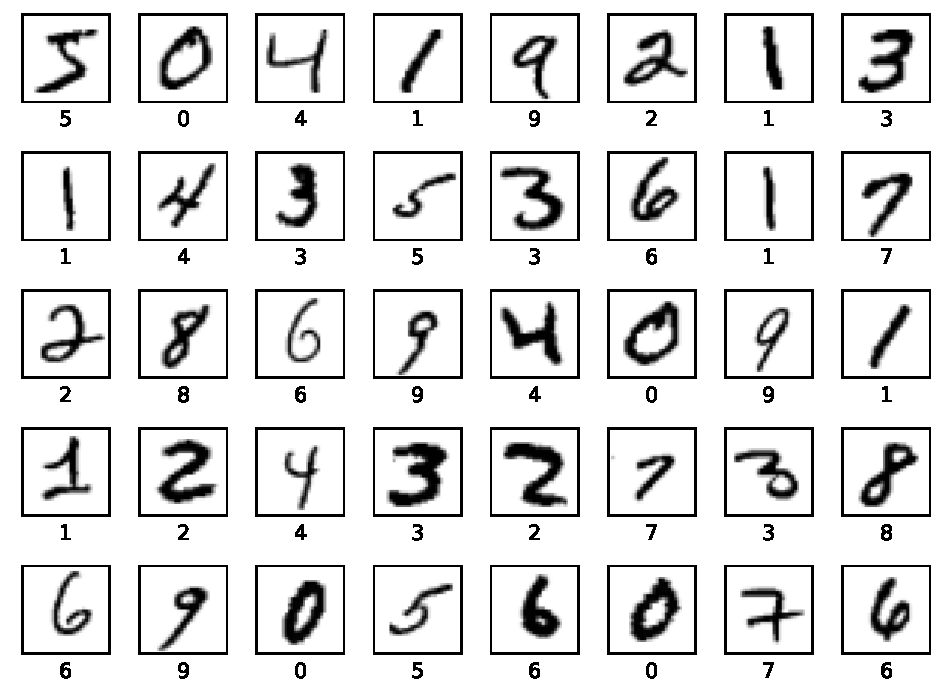
\includegraphics[width=0.6\textwidth]{chapters/Datasets/figures/MNIST.pdf}
    \fonte{From the author (2021)}
    \label{fig:dataset_mnist}
\end{figure}


\section{Fashion MNIST} \label{sec:fashion_mnist}
The simplicity of the \gls{MNIST} dataset makes it a very natural choice for benchmarking a Neural Network, however the data that it represents is also very simplistic \textbf{--} \textcite{mnistSOTA2013} were able to achieve a classification error lower than 0.3\% on the test set. The fact that \gls{MNIST} can be too easy has raised some questions about the usefulness of this dataset in benchmarking methods that scale to more complex tasks.

In response to these questions \textcite{fashionMNIST2017} proposed the Fashion MNIST dataset, arguing that \gls{MNIST} is too easy and cannot represent modern computer vision problems. Their goal was to replace \gls{MNIST} with a more robust dataset, without losing the simplicity of use that made the original so popular in the first place.

The Fashion MNIST dataset has all the same properties of \gls{MNIST}, it consists of 70,000 (60,000 training and 10,000 testing) $28{\times}28$ gray-scale images labelled from 0 to 9. The images however do not represent handwritten digits, they are instead preprocessed pictures of clothing items from the Zalando fashion company \cite{fashionMNIST2017}, the labels directly map to the type of clothing represented. Just like in \gls{MNIST}, the pixel values for the images are also inverted, the authors have made an effort to make the change of datasets as simple as just changing the link to get the files.

\autoref{fig:dataset_fashion_mnist} shows some labeled samples from this dataset, the pixel values are inverted for better visualization.
\begin{figure}[hbt]
    \centering
    \caption{Labeled samples from the Fashion MNIST dataset}
    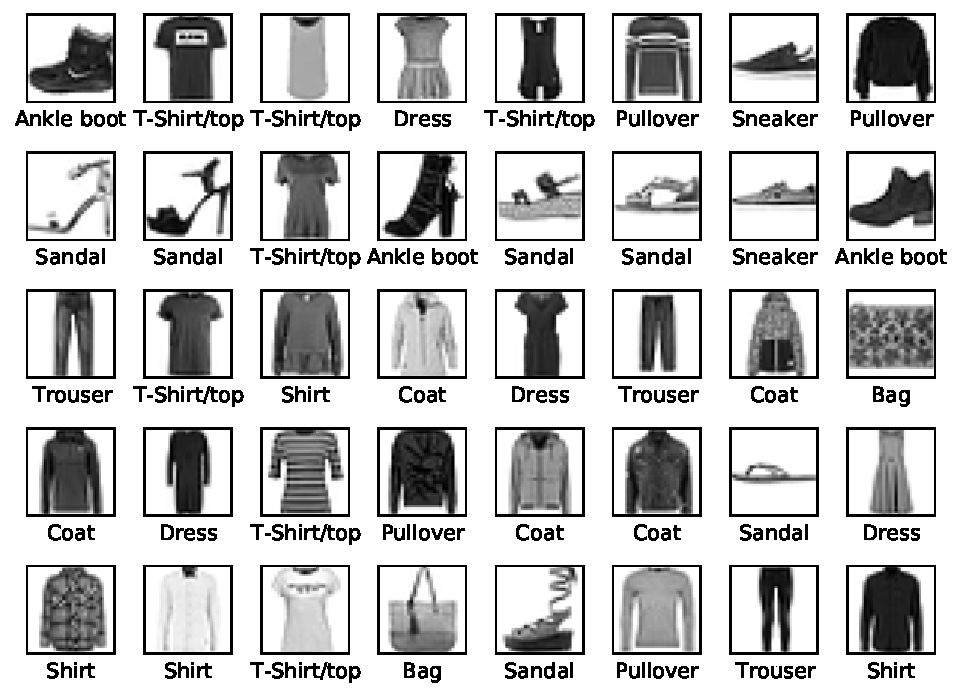
\includegraphics[width=0.7\textwidth]{chapters/Datasets/figures/Fashion_MNIST.pdf}
    \fonte{From the author (2021)}
    \label{fig:dataset_fashion_mnist}
\end{figure}


\section{CIFAR-10} \label{sec:cifar}
The \gls{CIFAR} datasets, \gls{CIFAR}-10 and \gls{CIFAR}-100, are two different subsets of the much larger 80 Million Tiny Images dataset, both are made of 60,000 (50,000 training and 10,000 testing) colored natural images of size $32{\times}32$ that were labeled by paid students to fit in a set of classes.

The images from \gls{CIFAR}-10 are divided into 10 classes with 6,000 images each, while \gls{CIFAR}-100 has 100 classes with 600 images each \cite{cifar2009}. For this document, only the \gls{CIFAR}-10 dataset was chosen for the experiments.

The \gls{CIFAR} datasets are another very popular choice for benchmarking neural networks, but given that they consist of colored images with increased resolution and more complex classes they offer considerably more challenge when compared to the \gls{MNIST} dataset. \autoref{fig:dataset_cifar10} shows examples of labeled samples taken from the \gls{CIFAR}-10 dataset.
\begin{figure}[hbt]
    \centering
    \caption{Labeled samples from CIFAR10 dataset}
    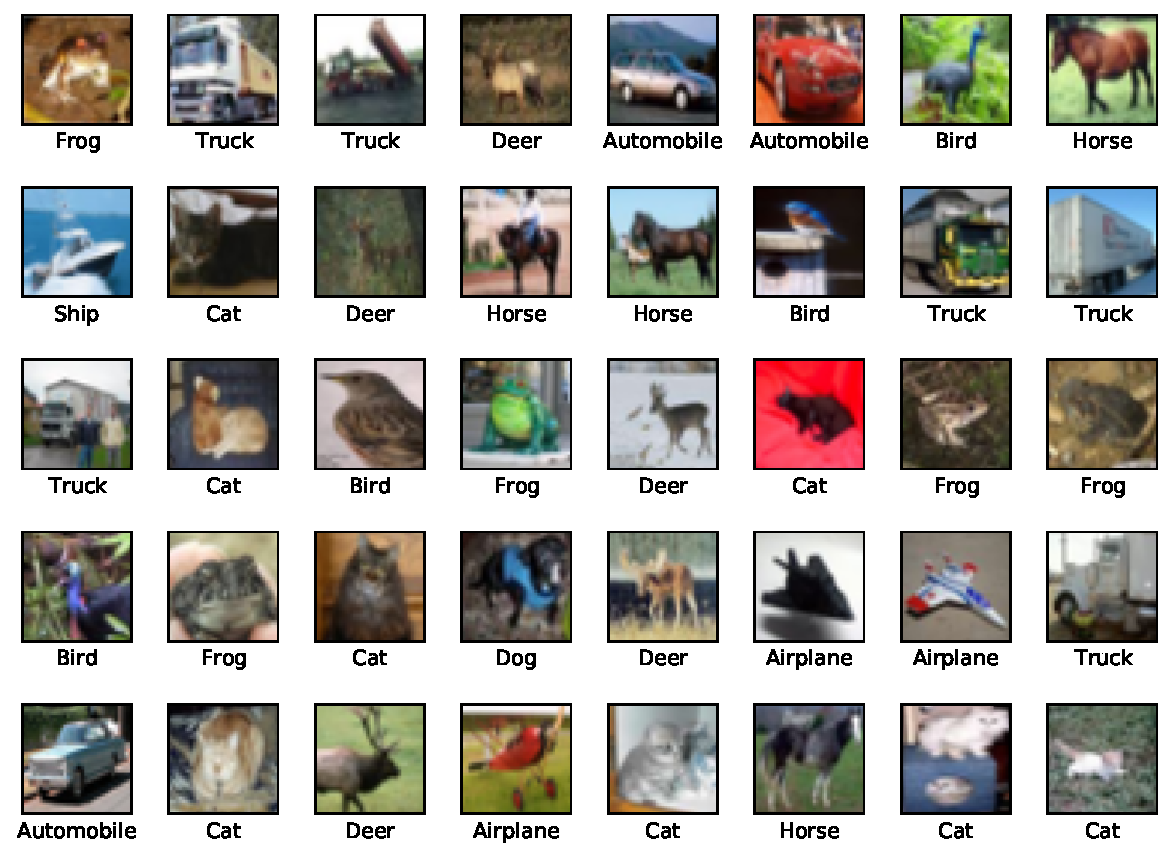
\includegraphics[width=0.7\textwidth]{chapters/Datasets/figures/CIFAR10.pdf}
    \fonte{From the author (2021)}
    \label{fig:dataset_cifar10}
\end{figure}



\section{Flowers} \label{sec:flowers}
The flowers dataset consists of $8,189$ high resolution images of 102 different categories of flowers, each category has from 40 to 250 different images \cite{flowers2008}. Samples from this dataset can be seen on \autoref{fig:dataset_flowers}

\begin{figure} [hbt]
    \centering
    \caption{Samples from the Flowers dataset}
    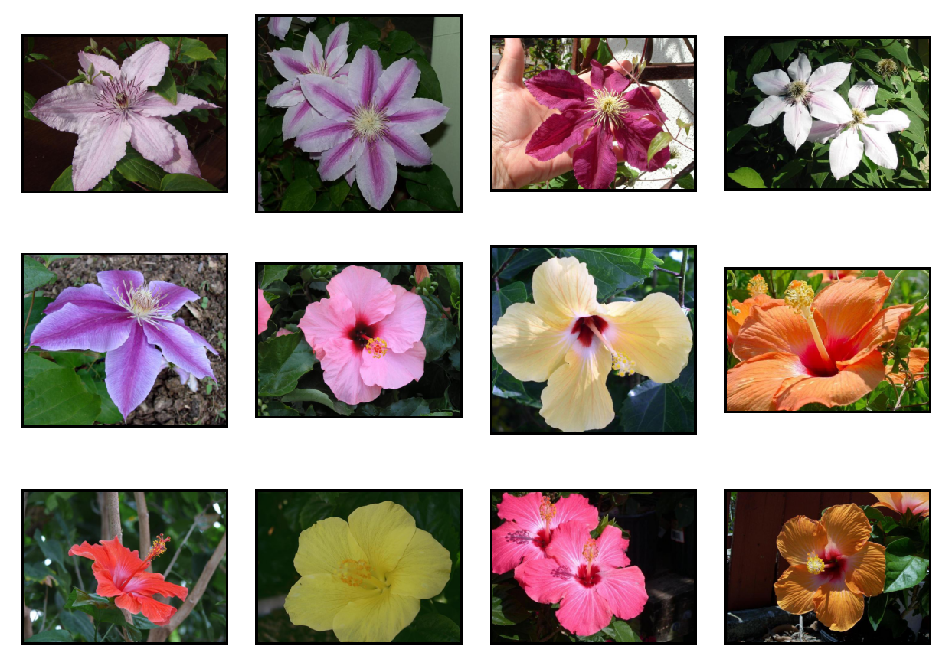
\includegraphics[width=0.8\textwidth]{chapters/Datasets/figures/Flowers.pdf}
    \fonte{From the author (2021)}
    \label{fig:dataset_flowers}
\end{figure}

\section{CelebA} \label{sec:celebA}
This is the largest dataset used in this document in terms of number of elements, it consists of $202,599$ pictures of faces of celebrities, all rescaled to size $178\times218$. All images are heavily annotated, having $40$ binary features (e.g. blonde hair, eyeglasses, wearing hat, young) and the positions of eyes, nose and mouth all labeled \cite{celebA2015}. However, for the purposes of this document the annotations will not be relevant. \autoref{fig:dataset_celeba} shows examples of pictures in this dataset.
\begin{figure}
    \centering
    \caption{Samples from the CelebA dataset}
    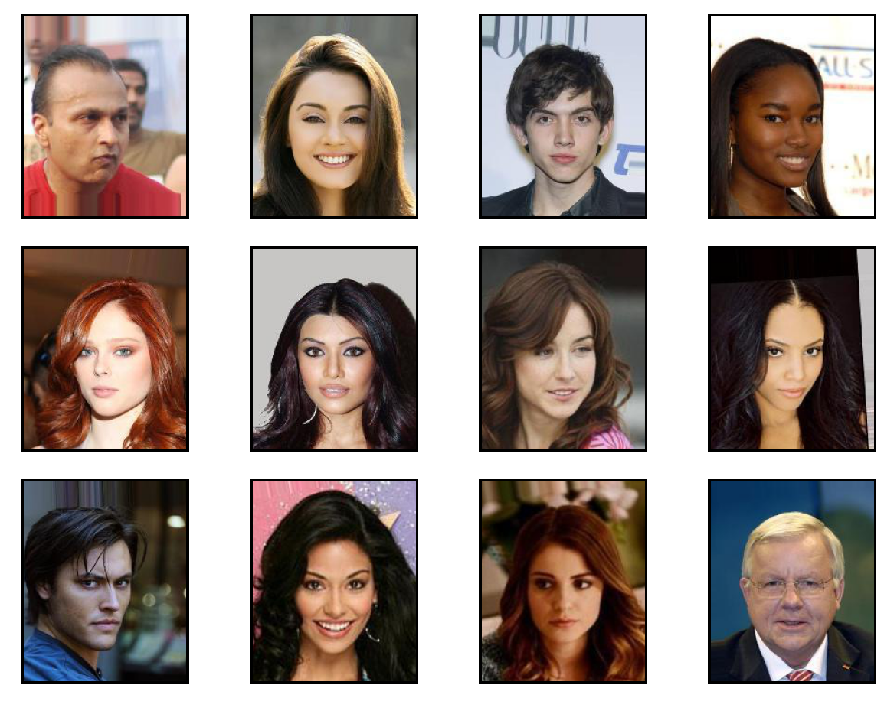
\includegraphics[width=0.8\textwidth]{chapters/Datasets/figures/CelebA.pdf}
    \fonte{From the author (2021)}
    \label{fig:dataset_celeba}
\end{figure}

\chapter{Datasets} \label{cha:datasets}
To understand the concepts explored in this document it is sometimes helpful to bring real world examples in order to represent the theoretical ideas in more familiar terms. This chapter will introduce the datasets relevant to this document, used for explaining the concepts, but mostly for performing the experiments that will be described in \autoref{cha:experiments}.

For any machine learning problem there is the desire to model something, some practical examples could be: how likely a person is to have a disease given a set of medical conditions; what type of animal an image represents; or what is the best move to make given a board position in chess. Whatever the underlying situation being modeled, it is necessary to have some data to build the model around.

This data can be obtained through self play (e.g. in Reinforcement Learning problems), but in the majority of cases it is given by a dataset. A dataset is simply a collection of samples from the situation being modeled, it does not contain all the possible values but, if sufficiently expansive, it should have enough samples to be a good representation of the distributions and particularities of the modeled situation. The goal of a dataset is to contain enough data, so that a machine learning algorithm trained on it can generalize well to data outside of it.

For neural networks a dataset is commonly divided into three groups: training, validation and test data. The training data is used in the learning process, it is what the network will see and will try to model, given this importance it is usually the largest chunk of a dataset. The validation data on the other hand is used to decide how to build the network and how to train the model, another way of saying this is that the training data is used to tune the network's parameters, while the validation data is used to tune the hyperparameters (see \autoref{sec:loss_&_gradient_descent}).

The validation process consists of training several models on the usually smaller validation data and seeing which set of hyperparameters produced the better results. One might wonder why would there be a need for this data and why not just use the training data instead? The main benefit of using a different set for validation is that validating on the training data has the risk of finding a set of hyperparameters that is particularly good on this data but that does not generalize well, using a separate validation data is a way to not overfit the hyperparameters to the training data and achieve better generalization.

The last chunk of a dataset, the test data, is used to validate the quality of the model and it's hability to generalize. This data should never be used to update either the parameters or hyperparameters, it should instead only be used as an evaluation tool, a way to estimate how well the model will perform on unseen data.

The next sections will explore the datasets relevant to the experiments made for this document. It is usual for datasets to already come separated into train and test data (the validation data is usually taken from a subset of the training data only if needed). This division will be mentioned for the described datasets, but it is relevant to note that any other divisions could also be obtained by combining and redistributing the data differently.


\section{MNIST} \label{sec:mnist}
\glsreset{MNIST}
Introduced in 1998 by \textcite{mnist1998}, the \gls{MNIST} is one of the most popular datasets in the field of machine learning, it's simplicity has made it a perfect choice as an introduction to deep learning and classification problems \cite{NN&DL2015}, but also as a benchmark for new techniques in serious research \textbf{--} some examples include \cite{dropout2012}, \cite{gans2014}, \cite{conditionalGAN2014} and \cite{adam2017}.

This dataset consists of 70,000 (60,000 training and 10,000 test) gray-scale images of handwritten digits, all images are of size $28{\times}28$ pixels and are labeled with the corresponding digit. The pixel values are inverted, this means that the strength of the strokes are represented with white pixels (values close to 255) against a black background (pixel value 0), this is however just how the data is represented numerically, for visualization purposes it is better to invert the colors as seen on \autoref{fig:dataset_mnist} \textbf{--} This figure shows some samples from this dataset along with the corresponding label.
\begin{figure}[hbt]
    \centering
    \caption{Labeled samples from the MNIST dataset}
    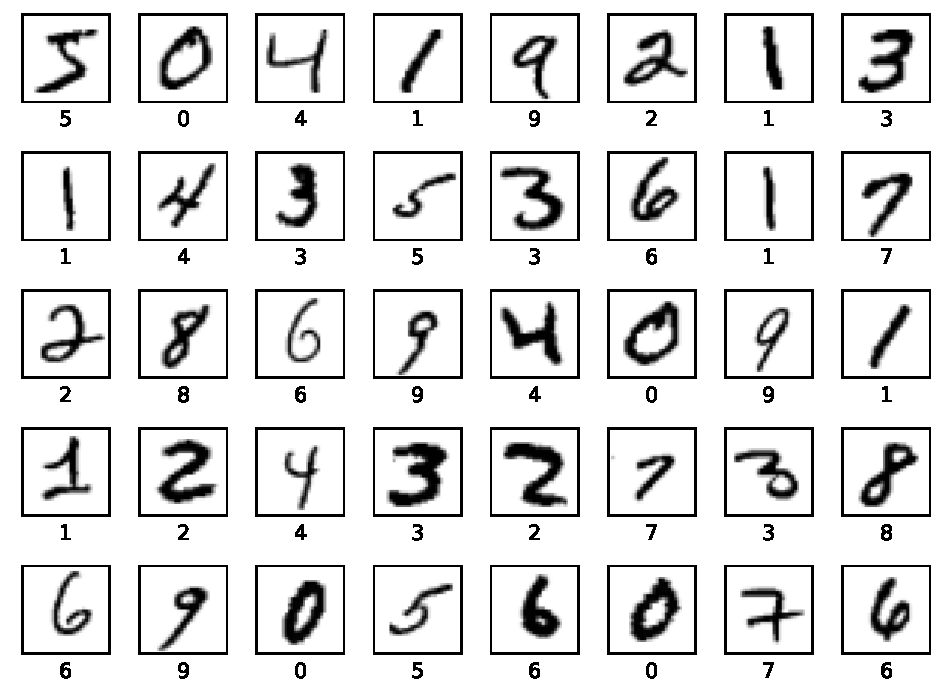
\includegraphics[width=0.6\textwidth]{chapters/Datasets/figures/MNIST.pdf}
    \fonte{From the author (2021)}
    \label{fig:dataset_mnist}
\end{figure}


\section{Fashion MNIST} \label{sec:fashion_mnist}
The simplicity of the \gls{MNIST} dataset makes it a very natural choice for benchmarking a Neural Network, however the data that it represents is also very simplistic \textbf{--} \textcite{mnistSOTA2013} were able to achieve a classification error lower than 0.3\% on the test set. The fact that \gls{MNIST} can be too easy has raised some questions about the usefulness of this dataset in benchmarking methods that scale to more complex tasks.

In response to these questions \textcite{fashionMNIST2017} proposed the Fashion MNIST dataset, arguing that \gls{MNIST} is too easy and cannot represent modern computer vision problems. Their goal was to replace \gls{MNIST} with a more robust dataset, without losing the simplicity of use that made the original so popular in the first place.

The Fashion MNIST dataset has all the same properties of \gls{MNIST}, it consists of 70,000 (60,000 training and 10,000 testing) $28{\times}28$ gray-scale images labelled from 0 to 9. The images however do not represent handwritten digits, they are instead preprocessed pictures of clothing items from the Zalando fashion company \cite{fashionMNIST2017}, the labels directly map to the type of clothing represented. Just like in \gls{MNIST}, the pixel values for the images are also inverted, the authors have made an effort to make the change of datasets as simple as just changing the link to get the files.

\autoref{fig:dataset_fashion_mnist} shows some labeled samples from this dataset, the pixel values are inverted for better visualization.
\begin{figure}[hbt]
    \centering
    \caption{Labeled samples from the Fashion MNIST dataset}
    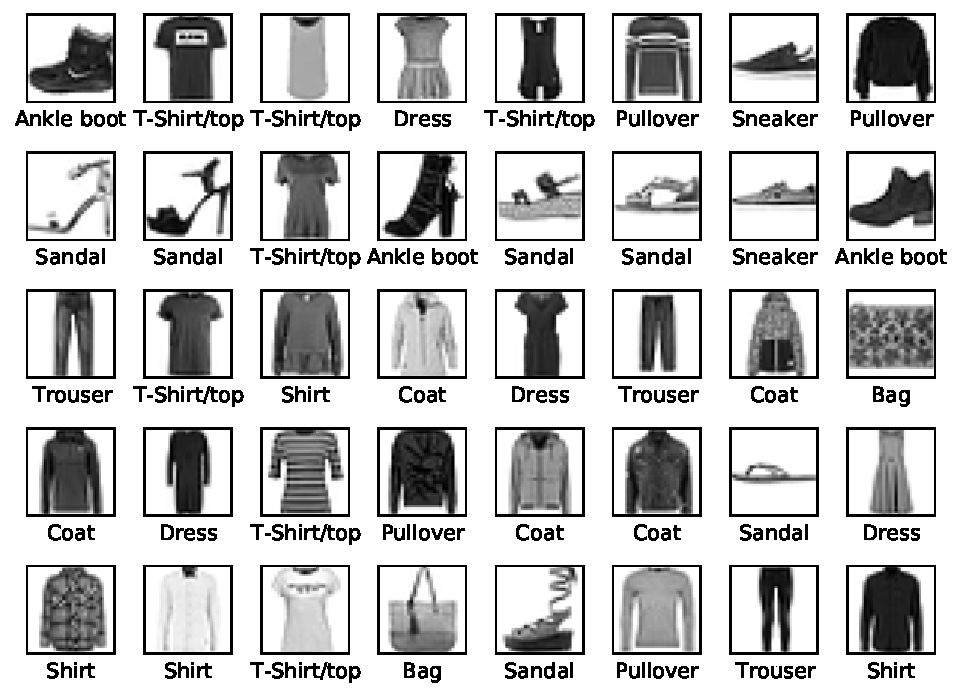
\includegraphics[width=0.7\textwidth]{chapters/Datasets/figures/Fashion_MNIST.pdf}
    \fonte{From the author (2021)}
    \label{fig:dataset_fashion_mnist}
\end{figure}


\section{CIFAR-10} \label{sec:cifar}
The \gls{CIFAR} datasets, \gls{CIFAR}-10 and \gls{CIFAR}-100, are two different subsets of the much larger 80 Million Tiny Images dataset, both are made of 60,000 (50,000 training and 10,000 testing) colored natural images of size $32{\times}32$ that were labeled by paid students to fit in a set of classes.

The images from \gls{CIFAR}-10 are divided into 10 classes with 6,000 images each, while \gls{CIFAR}-100 has 100 classes with 600 images each \cite{cifar2009}. For this document, only the \gls{CIFAR}-10 dataset was chosen for the experiments.

The \gls{CIFAR} datasets are another very popular choice for benchmarking neural networks, but given that they consist of colored images with increased resolution and more complex classes they offer considerably more challenge when compared to the \gls{MNIST} dataset. \autoref{fig:dataset_cifar10} shows examples of labeled samples taken from the \gls{CIFAR}-10 dataset.
\begin{figure}[hbt]
    \centering
    \caption{Labeled samples from CIFAR10 dataset}
    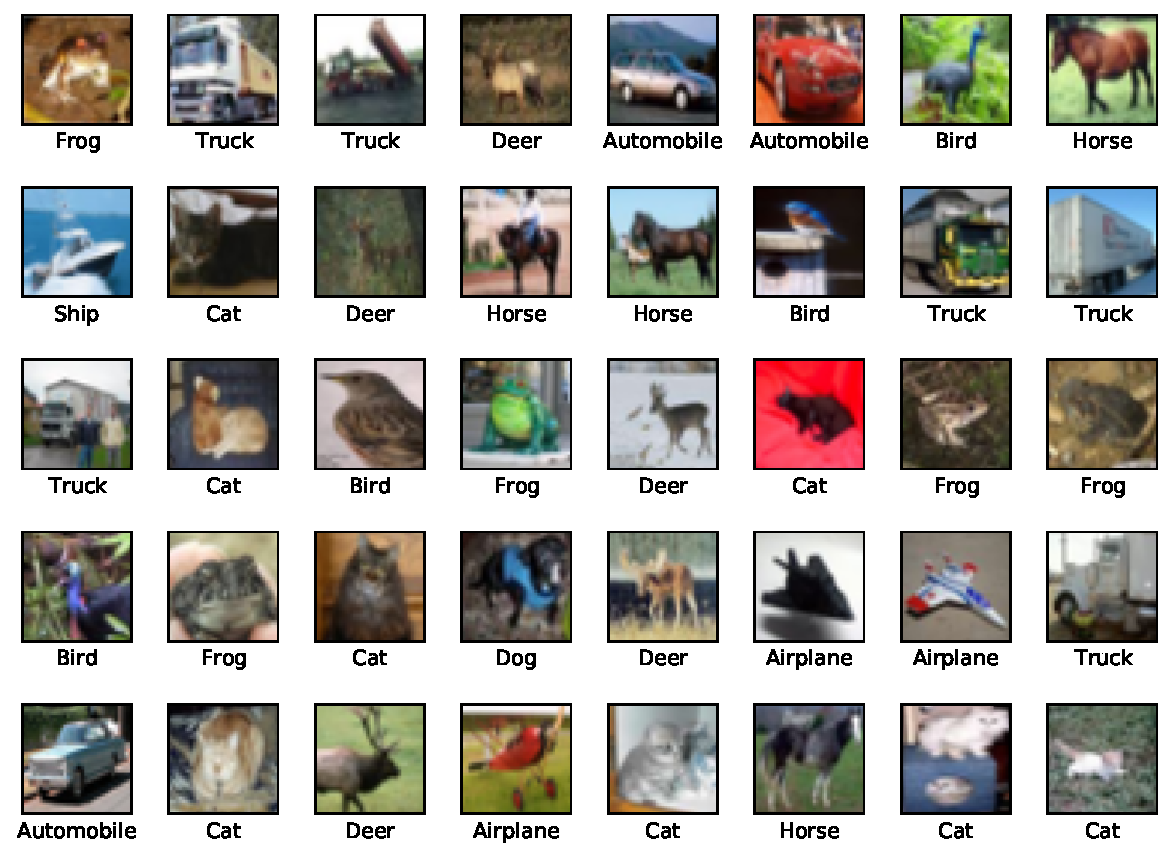
\includegraphics[width=0.7\textwidth]{chapters/Datasets/figures/CIFAR10.pdf}
    \fonte{From the author (2021)}
    \label{fig:dataset_cifar10}
\end{figure}



\section{Flowers} \label{sec:flowers}
The flowers dataset consists of $8,189$ high resolution images of 102 different categories of flowers, each category has from 40 to 250 different images \cite{flowers2008}. Samples from this dataset can be seen on \autoref{fig:dataset_flowers}

\begin{figure} [hbt]
    \centering
    \caption{Samples from the Flowers dataset}
    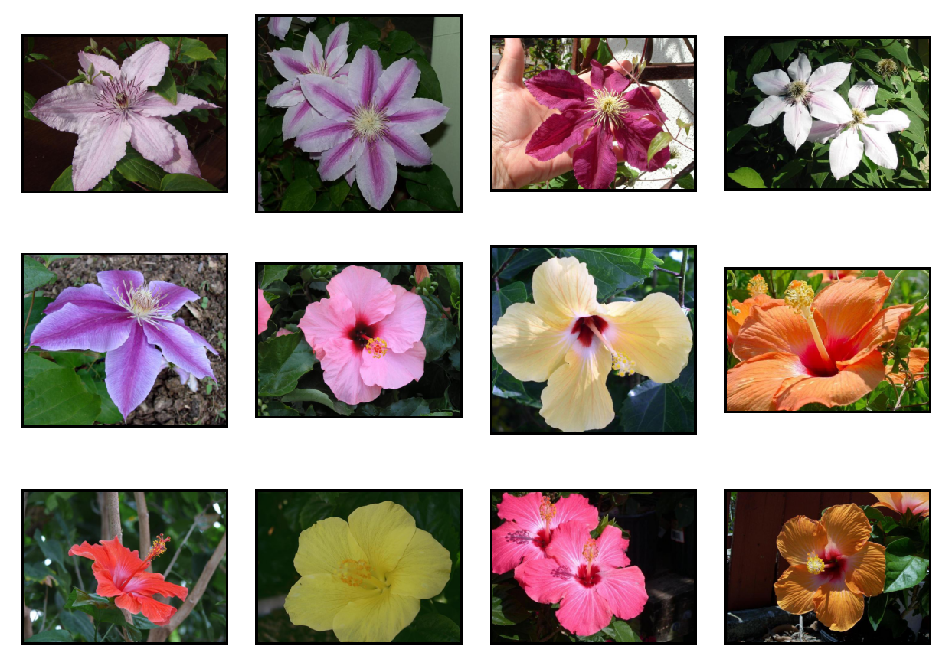
\includegraphics[width=0.8\textwidth]{chapters/Datasets/figures/Flowers.pdf}
    \fonte{From the author (2021)}
    \label{fig:dataset_flowers}
\end{figure}

\section{CelebA} \label{sec:celebA}
This is the largest dataset used in this document in terms of number of elements, it consists of $202,599$ pictures of faces of celebrities, all rescaled to size $178\times218$. All images are heavily annotated, having $40$ binary features (e.g. blonde hair, eyeglasses, wearing hat, young) and the positions of eyes, nose and mouth all labeled \cite{celebA2015}. However, for the purposes of this document the annotations will not be relevant. \autoref{fig:dataset_celeba} shows examples of pictures in this dataset.
\begin{figure}
    \centering
    \caption{Samples from the CelebA dataset}
    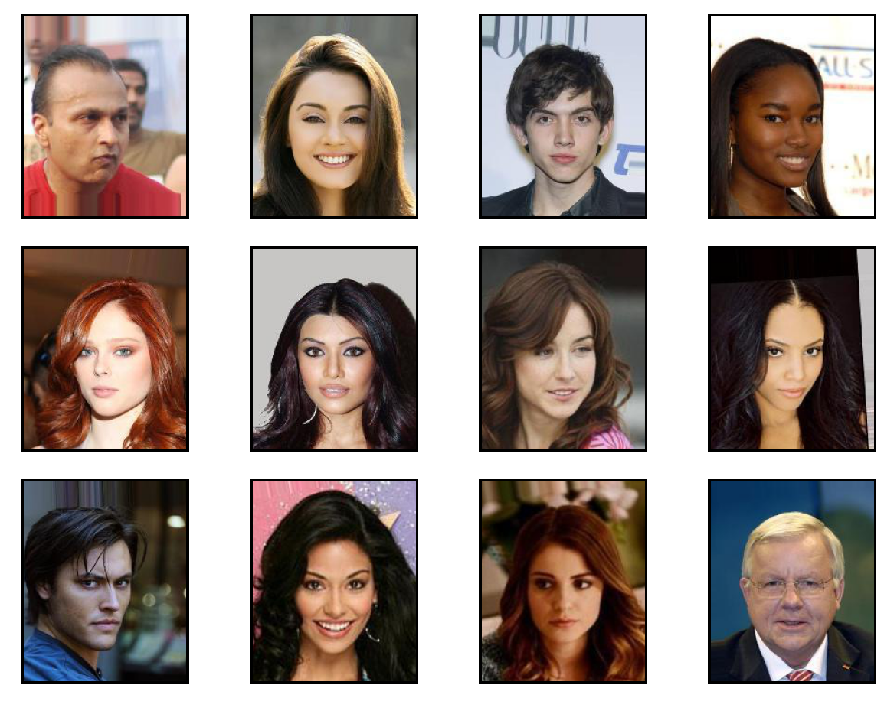
\includegraphics[width=0.8\textwidth]{chapters/Datasets/figures/CelebA.pdf}
    \fonte{From the author (2021)}
    \label{fig:dataset_celeba}
\end{figure}

\chapter{Datasets} \label{cha:datasets}
To understand the concepts explored in this document it is sometimes helpful to bring real world examples in order to represent the theoretical ideas in more familiar terms. This chapter will introduce the datasets relevant to this document, used for explaining the concepts, but mostly for performing the experiments that will be described in \autoref{cha:experiments}.

For any machine learning problem there is the desire to model something, some practical examples could be: how likely a person is to have a disease given a set of medical conditions; what type of animal an image represents; or what is the best move to make given a board position in chess. Whatever the underlying situation being modeled, it is necessary to have some data to build the model around.

This data can be obtained through self play (e.g. in Reinforcement Learning problems), but in the majority of cases it is given by a dataset. A dataset is simply a collection of samples from the situation being modeled, it does not contain all the possible values but, if sufficiently expansive, it should have enough samples to be a good representation of the distributions and particularities of the modeled situation. The goal of a dataset is to contain enough data, so that a machine learning algorithm trained on it can generalize well to data outside of it.

For neural networks a dataset is commonly divided into three groups: training, validation and test data. The training data is used in the learning process, it is what the network will see and will try to model, given this importance it is usually the largest chunk of a dataset. The validation data on the other hand is used to decide how to build the network and how to train the model, another way of saying this is that the training data is used to tune the network's parameters, while the validation data is used to tune the hyperparameters (see \autoref{sec:loss_&_gradient_descent}).

The validation process consists of training several models on the usually smaller validation data and seeing which set of hyperparameters produced the better results. One might wonder why would there be a need for this data and why not just use the training data instead? The main benefit of using a different set for validation is that validating on the training data has the risk of finding a set of hyperparameters that is particularly good on this data but that does not generalize well, using a separate validation data is a way to not overfit the hyperparameters to the training data and achieve better generalization.

The last chunk of a dataset, the test data, is used to validate the quality of the model and it's hability to generalize. This data should never be used to update either the parameters or hyperparameters, it should instead only be used as an evaluation tool, a way to estimate how well the model will perform on unseen data.

The next sections will explore the datasets relevant to the experiments made for this document. It is usual for datasets to already come separated into train and test data (the validation data is usually taken from a subset of the training data only if needed). This division will be mentioned for the described datasets, but it is relevant to note that any other divisions could also be obtained by combining and redistributing the data differently.


\section{MNIST} \label{sec:mnist}
\glsreset{MNIST}
Introduced in 1998 by \textcite{mnist1998}, the \gls{MNIST} is one of the most popular datasets in the field of machine learning, it's simplicity has made it a perfect choice as an introduction to deep learning and classification problems \cite{NN&DL2015}, but also as a benchmark for new techniques in serious research \textbf{--} some examples include \cite{dropout2012}, \cite{gans2014}, \cite{conditionalGAN2014} and \cite{adam2017}.

This dataset consists of 70,000 (60,000 training and 10,000 test) gray-scale images of handwritten digits, all images are of size $28{\times}28$ pixels and are labeled with the corresponding digit. The pixel values are inverted, this means that the strength of the strokes are represented with white pixels (values close to 255) against a black background (pixel value 0), this is however just how the data is represented numerically, for visualization purposes it is better to invert the colors as seen on \autoref{fig:dataset_mnist} \textbf{--} This figure shows some samples from this dataset along with the corresponding label.
\begin{figure}[hbt]
    \centering
    \caption{Labeled samples from the MNIST dataset}
    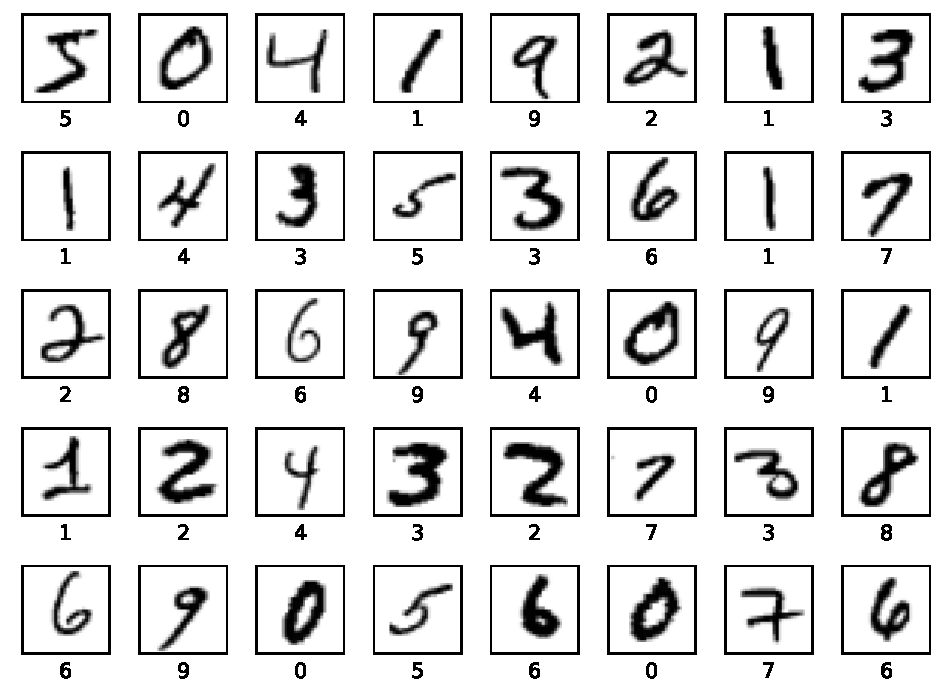
\includegraphics[width=0.6\textwidth]{chapters/Datasets/figures/MNIST.pdf}
    \fonte{From the author (2021)}
    \label{fig:dataset_mnist}
\end{figure}


\section{Fashion MNIST} \label{sec:fashion_mnist}
The simplicity of the \gls{MNIST} dataset makes it a very natural choice for benchmarking a Neural Network, however the data that it represents is also very simplistic \textbf{--} \textcite{mnistSOTA2013} were able to achieve a classification error lower than 0.3\% on the test set. The fact that \gls{MNIST} can be too easy has raised some questions about the usefulness of this dataset in benchmarking methods that scale to more complex tasks.

In response to these questions \textcite{fashionMNIST2017} proposed the Fashion MNIST dataset, arguing that \gls{MNIST} is too easy and cannot represent modern computer vision problems. Their goal was to replace \gls{MNIST} with a more robust dataset, without losing the simplicity of use that made the original so popular in the first place.

The Fashion MNIST dataset has all the same properties of \gls{MNIST}, it consists of 70,000 (60,000 training and 10,000 testing) $28{\times}28$ gray-scale images labelled from 0 to 9. The images however do not represent handwritten digits, they are instead preprocessed pictures of clothing items from the Zalando fashion company \cite{fashionMNIST2017}, the labels directly map to the type of clothing represented. Just like in \gls{MNIST}, the pixel values for the images are also inverted, the authors have made an effort to make the change of datasets as simple as just changing the link to get the files.

\autoref{fig:dataset_fashion_mnist} shows some labeled samples from this dataset, the pixel values are inverted for better visualization.
\begin{figure}[hbt]
    \centering
    \caption{Labeled samples from the Fashion MNIST dataset}
    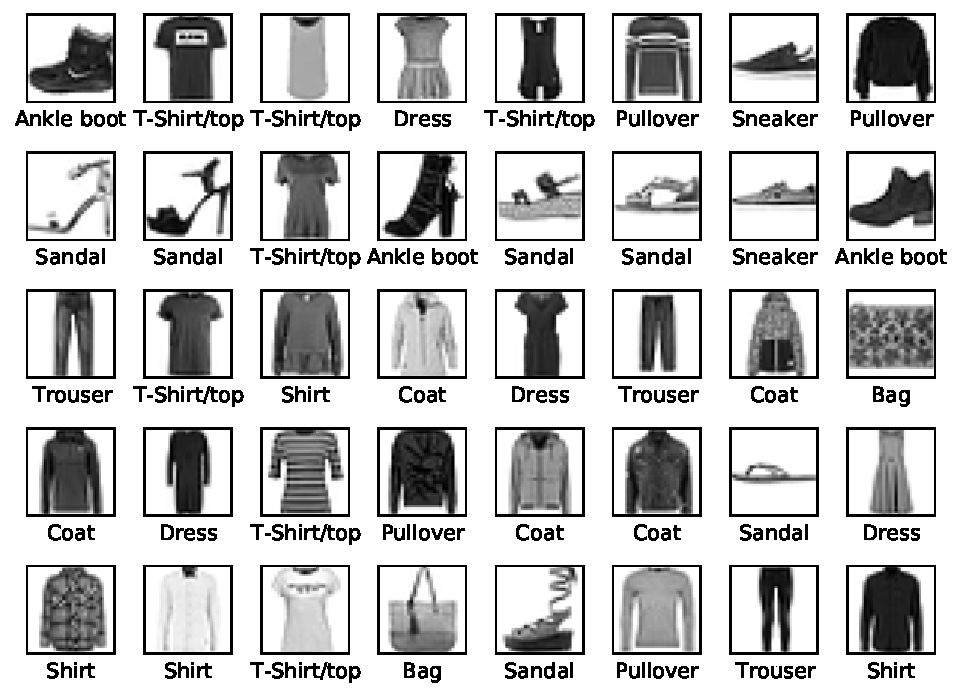
\includegraphics[width=0.7\textwidth]{chapters/Datasets/figures/Fashion_MNIST.pdf}
    \fonte{From the author (2021)}
    \label{fig:dataset_fashion_mnist}
\end{figure}


\section{CIFAR-10} \label{sec:cifar}
The \gls{CIFAR} datasets, \gls{CIFAR}-10 and \gls{CIFAR}-100, are two different subsets of the much larger 80 Million Tiny Images dataset, both are made of 60,000 (50,000 training and 10,000 testing) colored natural images of size $32{\times}32$ that were labeled by paid students to fit in a set of classes.

The images from \gls{CIFAR}-10 are divided into 10 classes with 6,000 images each, while \gls{CIFAR}-100 has 100 classes with 600 images each \cite{cifar2009}. For this document, only the \gls{CIFAR}-10 dataset was chosen for the experiments.

The \gls{CIFAR} datasets are another very popular choice for benchmarking neural networks, but given that they consist of colored images with increased resolution and more complex classes they offer considerably more challenge when compared to the \gls{MNIST} dataset. \autoref{fig:dataset_cifar10} shows examples of labeled samples taken from the \gls{CIFAR}-10 dataset.
\begin{figure}[hbt]
    \centering
    \caption{Labeled samples from CIFAR10 dataset}
    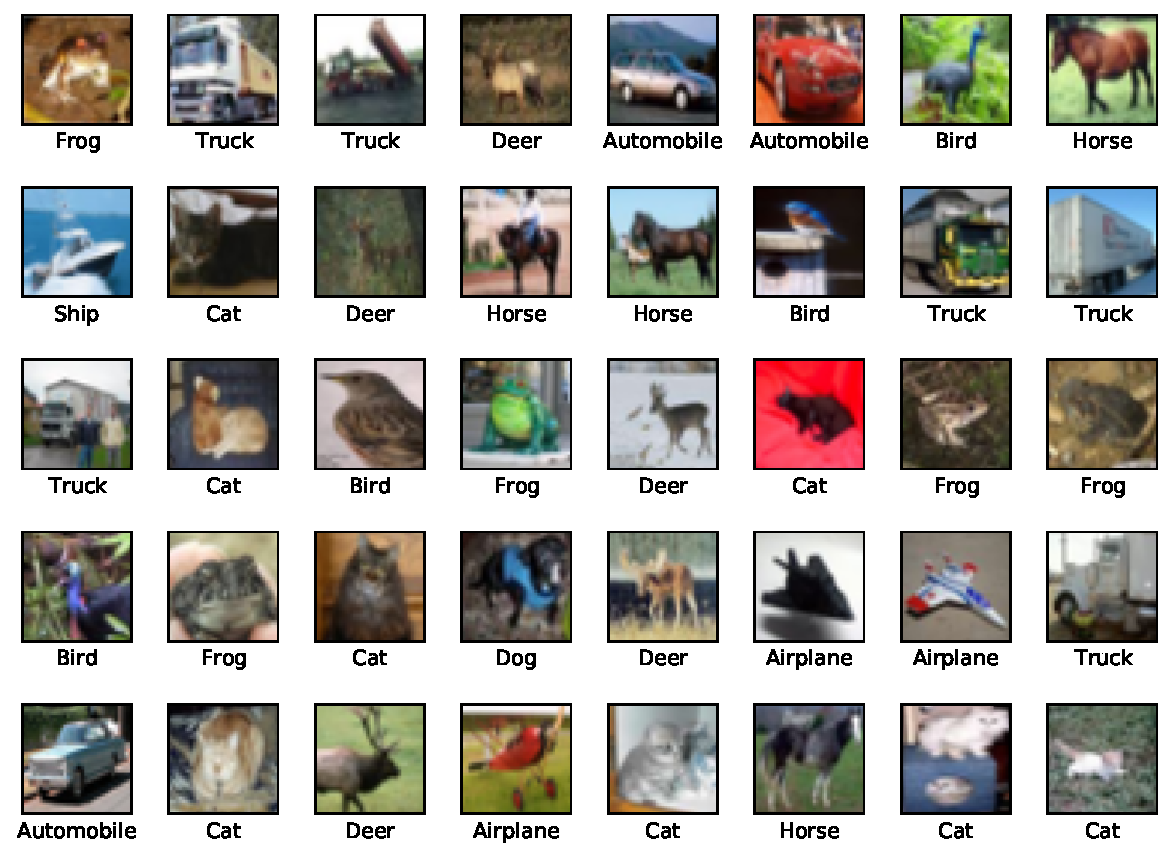
\includegraphics[width=0.7\textwidth]{chapters/Datasets/figures/CIFAR10.pdf}
    \fonte{From the author (2021)}
    \label{fig:dataset_cifar10}
\end{figure}



\section{Flowers} \label{sec:flowers}
The flowers dataset consists of $8,189$ high resolution images of 102 different categories of flowers, each category has from 40 to 250 different images \cite{flowers2008}. Samples from this dataset can be seen on \autoref{fig:dataset_flowers}

\begin{figure} [hbt]
    \centering
    \caption{Samples from the Flowers dataset}
    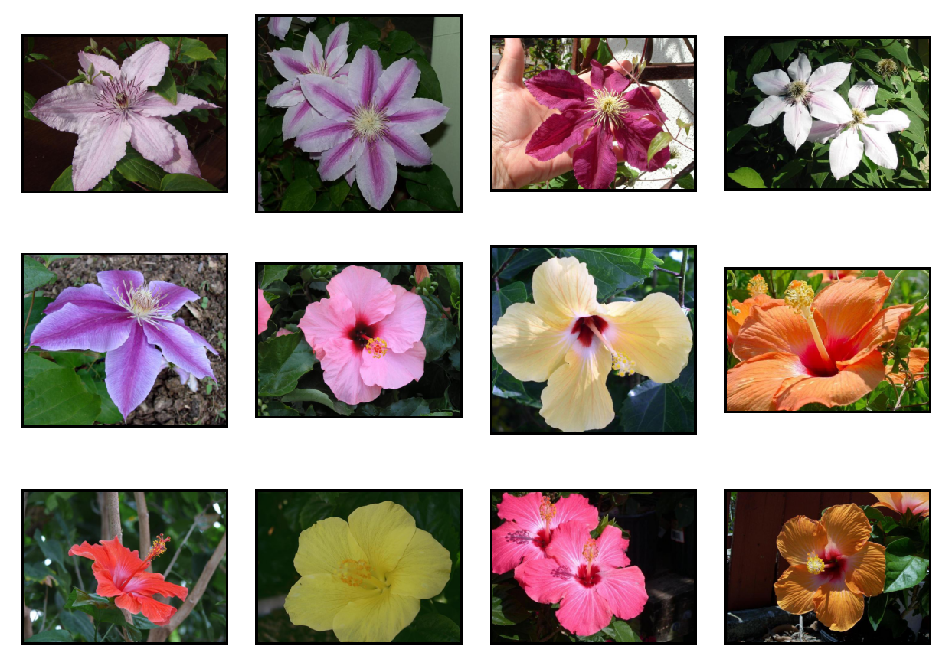
\includegraphics[width=0.8\textwidth]{chapters/Datasets/figures/Flowers.pdf}
    \fonte{From the author (2021)}
    \label{fig:dataset_flowers}
\end{figure}

\section{CelebA} \label{sec:celebA}
This is the largest dataset used in this document in terms of number of elements, it consists of $202,599$ pictures of faces of celebrities, all rescaled to size $178\times218$. All images are heavily annotated, having $40$ binary features (e.g. blonde hair, eyeglasses, wearing hat, young) and the positions of eyes, nose and mouth all labeled \cite{celebA2015}. However, for the purposes of this document the annotations will not be relevant. \autoref{fig:dataset_celeba} shows examples of pictures in this dataset.
\begin{figure}
    \centering
    \caption{Samples from the CelebA dataset}
    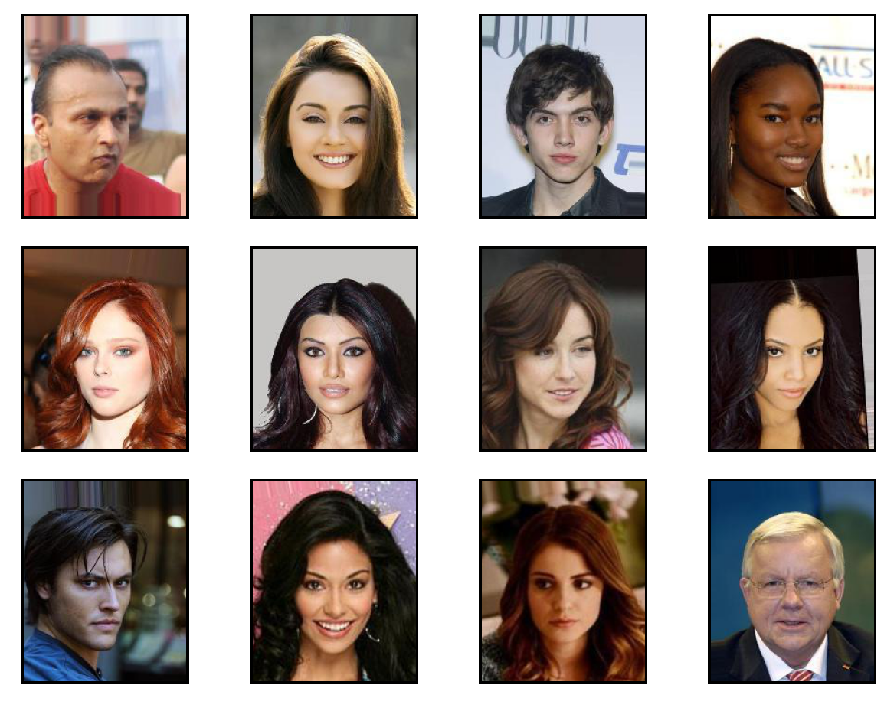
\includegraphics[width=0.8\textwidth]{chapters/Datasets/figures/CelebA.pdf}
    \fonte{From the author (2021)}
    \label{fig:dataset_celeba}
\end{figure}

\chapter{Datasets} \label{cha:datasets}
To understand the concepts explored in this document it is sometimes helpful to bring real world examples in order to represent the theoretical ideas in more familiar terms. This chapter will introduce the datasets relevant to this document, used for explaining the concepts, but mostly for performing the experiments that will be described in \autoref{cha:experiments}.

For any machine learning problem there is the desire to model something, some practical examples could be: how likely a person is to have a disease given a set of medical conditions; what type of animal an image represents; or what is the best move to make given a board position in chess. Whatever the underlying situation being modeled, it is necessary to have some data to build the model around.

This data can be obtained through self play (e.g. in Reinforcement Learning problems), but in the majority of cases it is given by a dataset. A dataset is simply a collection of samples from the situation being modeled, it does not contain all the possible values but, if sufficiently expansive, it should have enough samples to be a good representation of the distributions and particularities of the modeled situation. The goal of a dataset is to contain enough data, so that a machine learning algorithm trained on it can generalize well to data outside of it.

For neural networks a dataset is commonly divided into three groups: training, validation and test data. The training data is used in the learning process, it is what the network will see and will try to model, given this importance it is usually the largest chunk of a dataset. The validation data on the other hand is used to decide how to build the network and how to train the model, another way of saying this is that the training data is used to tune the network's parameters, while the validation data is used to tune the hyperparameters (see \autoref{sec:loss_&_gradient_descent}).

The validation process consists of training several models on the usually smaller validation data and seeing which set of hyperparameters produced the better results. One might wonder why would there be a need for this data and why not just use the training data instead? The main benefit of using a different set for validation is that validating on the training data has the risk of finding a set of hyperparameters that is particularly good on this data but that does not generalize well, using a separate validation data is a way to not overfit the hyperparameters to the training data and achieve better generalization.

The last chunk of a dataset, the test data, is used to validate the quality of the model and it's hability to generalize. This data should never be used to update either the parameters or hyperparameters, it should instead only be used as an evaluation tool, a way to estimate how well the model will perform on unseen data.

The next sections will explore the datasets relevant to the experiments made for this document. It is usual for datasets to already come separated into train and test data (the validation data is usually taken from a subset of the training data only if needed). This division will be mentioned for the described datasets, but it is relevant to note that any other divisions could also be obtained by combining and redistributing the data differently.


\section{MNIST} \label{sec:mnist}
\glsreset{MNIST}
Introduced in 1998 by \textcite{mnist1998}, the \gls{MNIST} is one of the most popular datasets in the field of machine learning, it's simplicity has made it a perfect choice as an introduction to deep learning and classification problems \cite{NN&DL2015}, but also as a benchmark for new techniques in serious research \textbf{--} some examples include \cite{dropout2012}, \cite{gans2014}, \cite{conditionalGAN2014} and \cite{adam2017}.

This dataset consists of 70,000 (60,000 training and 10,000 test) gray-scale images of handwritten digits, all images are of size $28{\times}28$ pixels and are labeled with the corresponding digit. The pixel values are inverted, this means that the strength of the strokes are represented with white pixels (values close to 255) against a black background (pixel value 0), this is however just how the data is represented numerically, for visualization purposes it is better to invert the colors as seen on \autoref{fig:dataset_mnist} \textbf{--} This figure shows some samples from this dataset along with the corresponding label.
\begin{figure}[hbt]
    \centering
    \caption{Labeled samples from the MNIST dataset}
    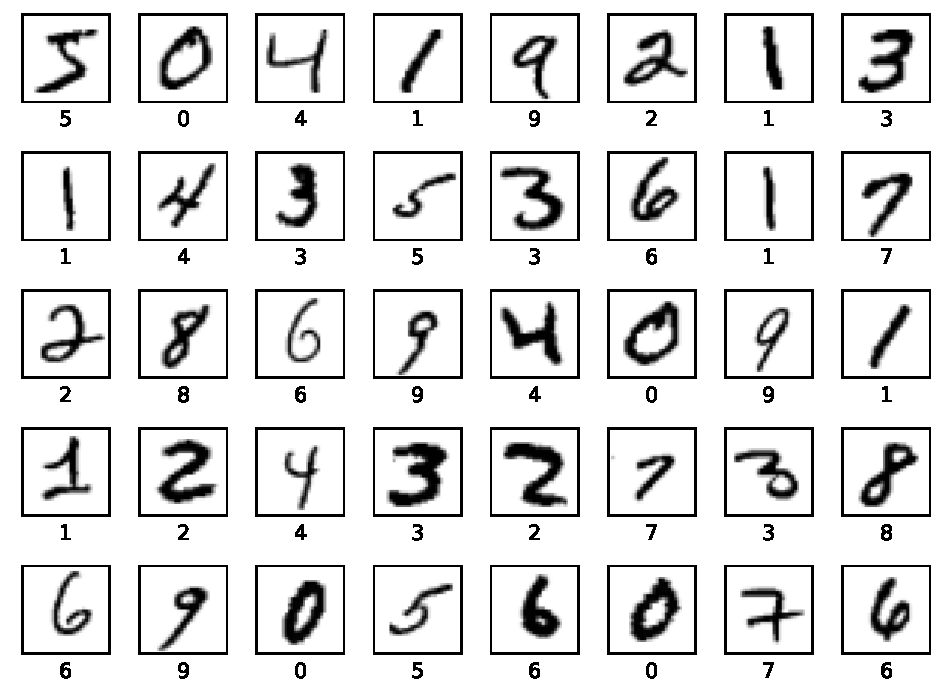
\includegraphics[width=0.6\textwidth]{chapters/Datasets/figures/MNIST.pdf}
    \fonte{From the author (2021)}
    \label{fig:dataset_mnist}
\end{figure}


\section{Fashion MNIST} \label{sec:fashion_mnist}
The simplicity of the \gls{MNIST} dataset makes it a very natural choice for benchmarking a Neural Network, however the data that it represents is also very simplistic \textbf{--} \textcite{mnistSOTA2013} were able to achieve a classification error lower than 0.3\% on the test set. The fact that \gls{MNIST} can be too easy has raised some questions about the usefulness of this dataset in benchmarking methods that scale to more complex tasks.

In response to these questions \textcite{fashionMNIST2017} proposed the Fashion MNIST dataset, arguing that \gls{MNIST} is too easy and cannot represent modern computer vision problems. Their goal was to replace \gls{MNIST} with a more robust dataset, without losing the simplicity of use that made the original so popular in the first place.

The Fashion MNIST dataset has all the same properties of \gls{MNIST}, it consists of 70,000 (60,000 training and 10,000 testing) $28{\times}28$ gray-scale images labelled from 0 to 9. The images however do not represent handwritten digits, they are instead preprocessed pictures of clothing items from the Zalando fashion company \cite{fashionMNIST2017}, the labels directly map to the type of clothing represented. Just like in \gls{MNIST}, the pixel values for the images are also inverted, the authors have made an effort to make the change of datasets as simple as just changing the link to get the files.

\autoref{fig:dataset_fashion_mnist} shows some labeled samples from this dataset, the pixel values are inverted for better visualization.
\begin{figure}[hbt]
    \centering
    \caption{Labeled samples from the Fashion MNIST dataset}
    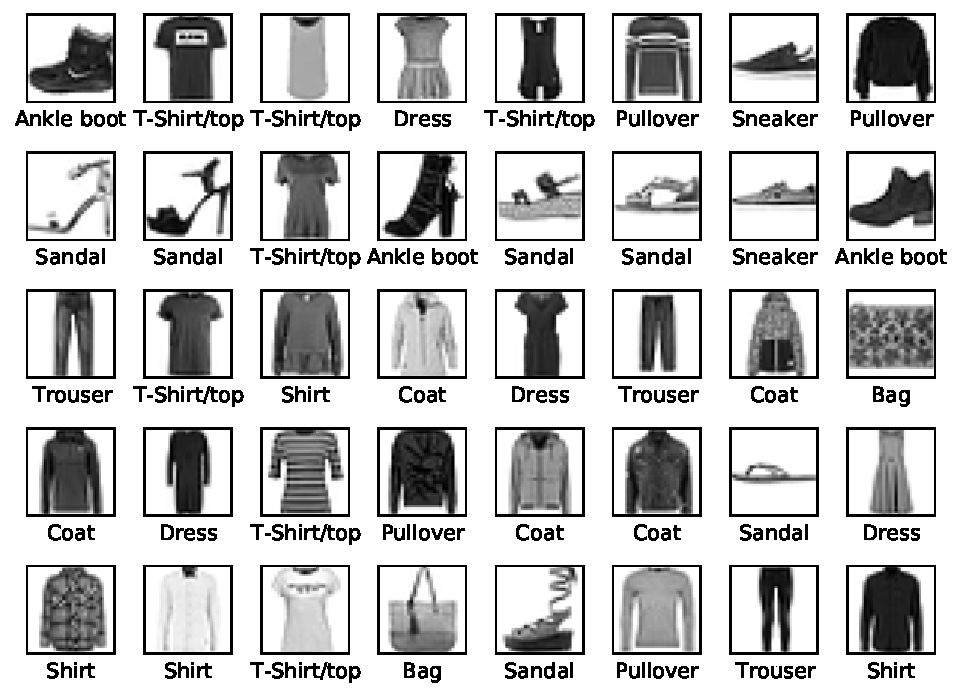
\includegraphics[width=0.7\textwidth]{chapters/Datasets/figures/Fashion_MNIST.pdf}
    \fonte{From the author (2021)}
    \label{fig:dataset_fashion_mnist}
\end{figure}


\section{CIFAR-10} \label{sec:cifar}
The \gls{CIFAR} datasets, \gls{CIFAR}-10 and \gls{CIFAR}-100, are two different subsets of the much larger 80 Million Tiny Images dataset, both are made of 60,000 (50,000 training and 10,000 testing) colored natural images of size $32{\times}32$ that were labeled by paid students to fit in a set of classes.

The images from \gls{CIFAR}-10 are divided into 10 classes with 6,000 images each, while \gls{CIFAR}-100 has 100 classes with 600 images each \cite{cifar2009}. For this document, only the \gls{CIFAR}-10 dataset was chosen for the experiments.

The \gls{CIFAR} datasets are another very popular choice for benchmarking neural networks, but given that they consist of colored images with increased resolution and more complex classes they offer considerably more challenge when compared to the \gls{MNIST} dataset. \autoref{fig:dataset_cifar10} shows examples of labeled samples taken from the \gls{CIFAR}-10 dataset.
\begin{figure}[hbt]
    \centering
    \caption{Labeled samples from CIFAR10 dataset}
    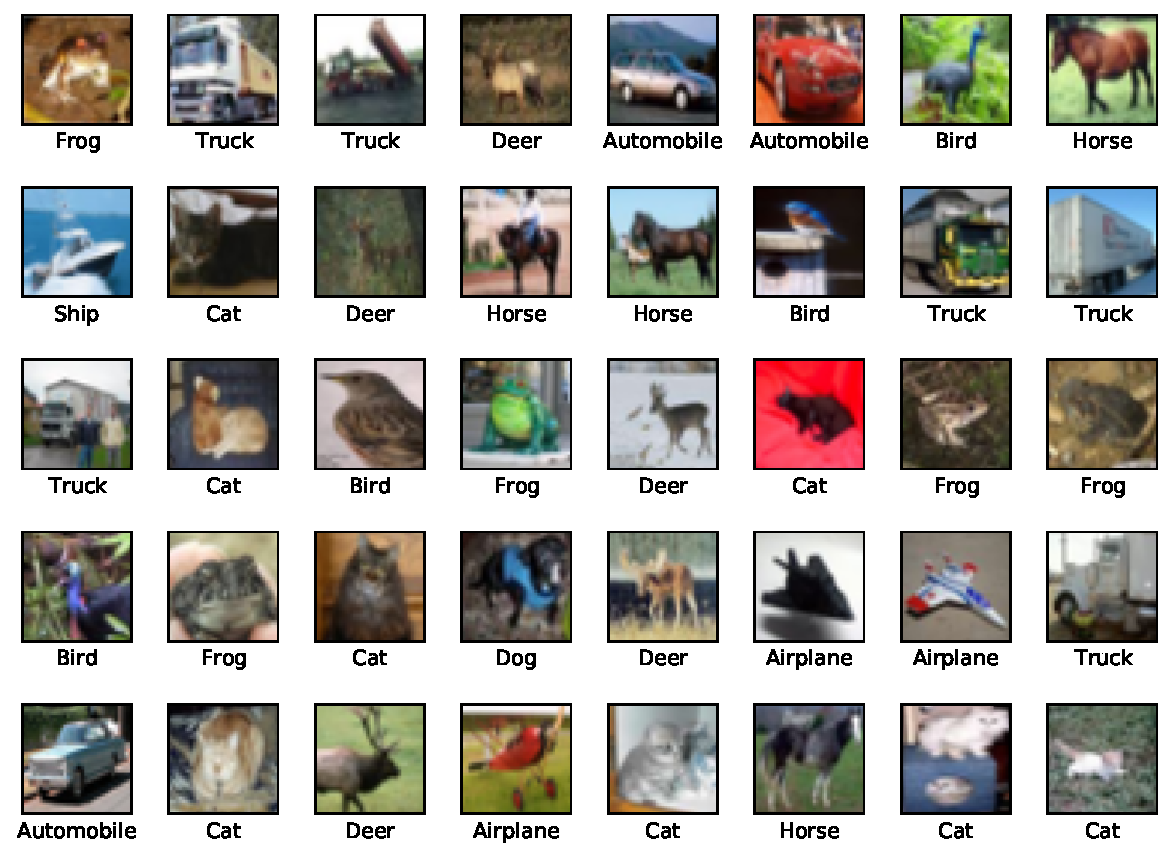
\includegraphics[width=0.7\textwidth]{chapters/Datasets/figures/CIFAR10.pdf}
    \fonte{From the author (2021)}
    \label{fig:dataset_cifar10}
\end{figure}



\section{Flowers} \label{sec:flowers}
The flowers dataset consists of $8,189$ high resolution images of 102 different categories of flowers, each category has from 40 to 250 different images \cite{flowers2008}. Samples from this dataset can be seen on \autoref{fig:dataset_flowers}

\begin{figure} [hbt]
    \centering
    \caption{Samples from the Flowers dataset}
    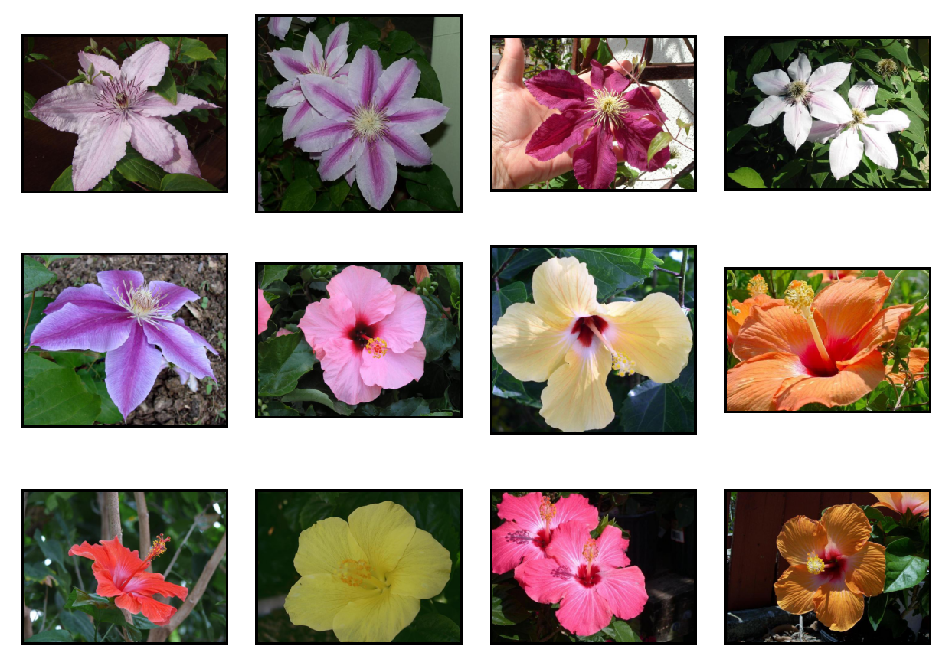
\includegraphics[width=0.8\textwidth]{chapters/Datasets/figures/Flowers.pdf}
    \fonte{From the author (2021)}
    \label{fig:dataset_flowers}
\end{figure}

\section{CelebA} \label{sec:celebA}
This is the largest dataset used in this document in terms of number of elements, it consists of $202,599$ pictures of faces of celebrities, all rescaled to size $178\times218$. All images are heavily annotated, having $40$ binary features (e.g. blonde hair, eyeglasses, wearing hat, young) and the positions of eyes, nose and mouth all labeled \cite{celebA2015}. However, for the purposes of this document the annotations will not be relevant. \autoref{fig:dataset_celeba} shows examples of pictures in this dataset.
\begin{figure}
    \centering
    \caption{Samples from the CelebA dataset}
    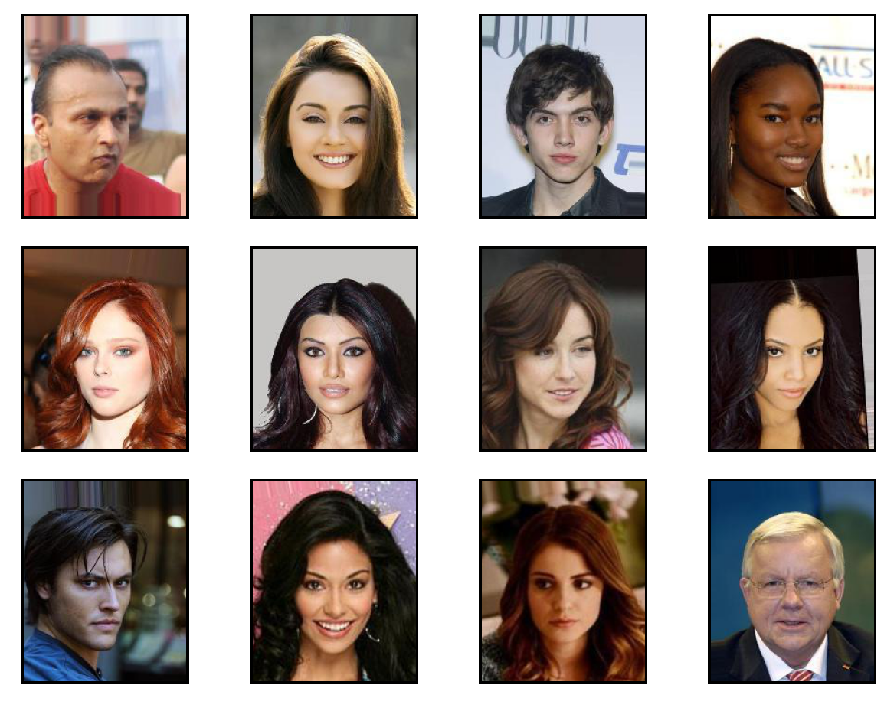
\includegraphics[width=0.8\textwidth]{chapters/Datasets/figures/CelebA.pdf}
    \fonte{From the author (2021)}
    \label{fig:dataset_celeba}
\end{figure}

\chapter{Datasets} \label{cha:datasets}
To understand the concepts explored in this document it is sometimes helpful to bring real world examples in order to represent the theoretical ideas in more familiar terms. This chapter will introduce the datasets relevant to this document, used for explaining the concepts, but mostly for performing the experiments that will be described in \autoref{cha:experiments}.

For any machine learning problem there is the desire to model something, some practical examples could be: how likely a person is to have a disease given a set of medical conditions; what type of animal an image represents; or what is the best move to make given a board position in chess. Whatever the underlying situation being modeled, it is necessary to have some data to build the model around.

This data can be obtained through self play (e.g. in Reinforcement Learning problems), but in the majority of cases it is given by a dataset. A dataset is simply a collection of samples from the situation being modeled, it does not contain all the possible values but, if sufficiently expansive, it should have enough samples to be a good representation of the distributions and particularities of the modeled situation. The goal of a dataset is to contain enough data, so that a machine learning algorithm trained on it can generalize well to data outside of it.

For neural networks a dataset is commonly divided into three groups: training, validation and test data. The training data is used in the learning process, it is what the network will see and will try to model, given this importance it is usually the largest chunk of a dataset. The validation data on the other hand is used to decide how to build the network and how to train the model, another way of saying this is that the training data is used to tune the network's parameters, while the validation data is used to tune the hyperparameters (see \autoref{sec:loss_&_gradient_descent}).

The validation process consists of training several models on the usually smaller validation data and seeing which set of hyperparameters produced the better results. One might wonder why would there be a need for this data and why not just use the training data instead? The main benefit of using a different set for validation is that validating on the training data has the risk of finding a set of hyperparameters that is particularly good on this data but that does not generalize well, using a separate validation data is a way to not overfit the hyperparameters to the training data and achieve better generalization.

The last chunk of a dataset, the test data, is used to validate the quality of the model and it's hability to generalize. This data should never be used to update either the parameters or hyperparameters, it should instead only be used as an evaluation tool, a way to estimate how well the model will perform on unseen data.

The next sections will explore the datasets relevant to the experiments made for this document. It is usual for datasets to already come separated into train and test data (the validation data is usually taken from a subset of the training data only if needed). This division will be mentioned for the described datasets, but it is relevant to note that any other divisions could also be obtained by combining and redistributing the data differently.


\section{MNIST} \label{sec:mnist}
\glsreset{MNIST}
Introduced in 1998 by \textcite{mnist1998}, the \gls{MNIST} is one of the most popular datasets in the field of machine learning, it's simplicity has made it a perfect choice as an introduction to deep learning and classification problems \cite{NN&DL2015}, but also as a benchmark for new techniques in serious research \textbf{--} some examples include \cite{dropout2012}, \cite{gans2014}, \cite{conditionalGAN2014} and \cite{adam2017}.

This dataset consists of 70,000 (60,000 training and 10,000 test) gray-scale images of handwritten digits, all images are of size $28{\times}28$ pixels and are labeled with the corresponding digit. The pixel values are inverted, this means that the strength of the strokes are represented with white pixels (values close to 255) against a black background (pixel value 0), this is however just how the data is represented numerically, for visualization purposes it is better to invert the colors as seen on \autoref{fig:dataset_mnist} \textbf{--} This figure shows some samples from this dataset along with the corresponding label.
\begin{figure}[hbt]
    \centering
    \caption{Labeled samples from the MNIST dataset}
    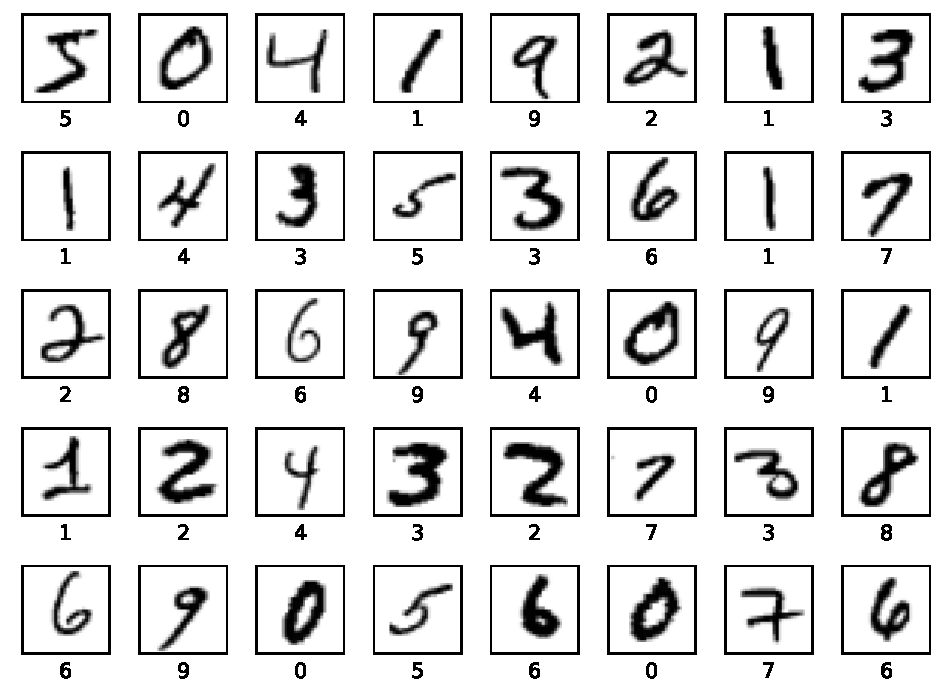
\includegraphics[width=0.6\textwidth]{chapters/Datasets/figures/MNIST.pdf}
    \fonte{From the author (2021)}
    \label{fig:dataset_mnist}
\end{figure}


\section{Fashion MNIST} \label{sec:fashion_mnist}
The simplicity of the \gls{MNIST} dataset makes it a very natural choice for benchmarking a Neural Network, however the data that it represents is also very simplistic \textbf{--} \textcite{mnistSOTA2013} were able to achieve a classification error lower than 0.3\% on the test set. The fact that \gls{MNIST} can be too easy has raised some questions about the usefulness of this dataset in benchmarking methods that scale to more complex tasks.

In response to these questions \textcite{fashionMNIST2017} proposed the Fashion MNIST dataset, arguing that \gls{MNIST} is too easy and cannot represent modern computer vision problems. Their goal was to replace \gls{MNIST} with a more robust dataset, without losing the simplicity of use that made the original so popular in the first place.

The Fashion MNIST dataset has all the same properties of \gls{MNIST}, it consists of 70,000 (60,000 training and 10,000 testing) $28{\times}28$ gray-scale images labelled from 0 to 9. The images however do not represent handwritten digits, they are instead preprocessed pictures of clothing items from the Zalando fashion company \cite{fashionMNIST2017}, the labels directly map to the type of clothing represented. Just like in \gls{MNIST}, the pixel values for the images are also inverted, the authors have made an effort to make the change of datasets as simple as just changing the link to get the files.

\autoref{fig:dataset_fashion_mnist} shows some labeled samples from this dataset, the pixel values are inverted for better visualization.
\begin{figure}[hbt]
    \centering
    \caption{Labeled samples from the Fashion MNIST dataset}
    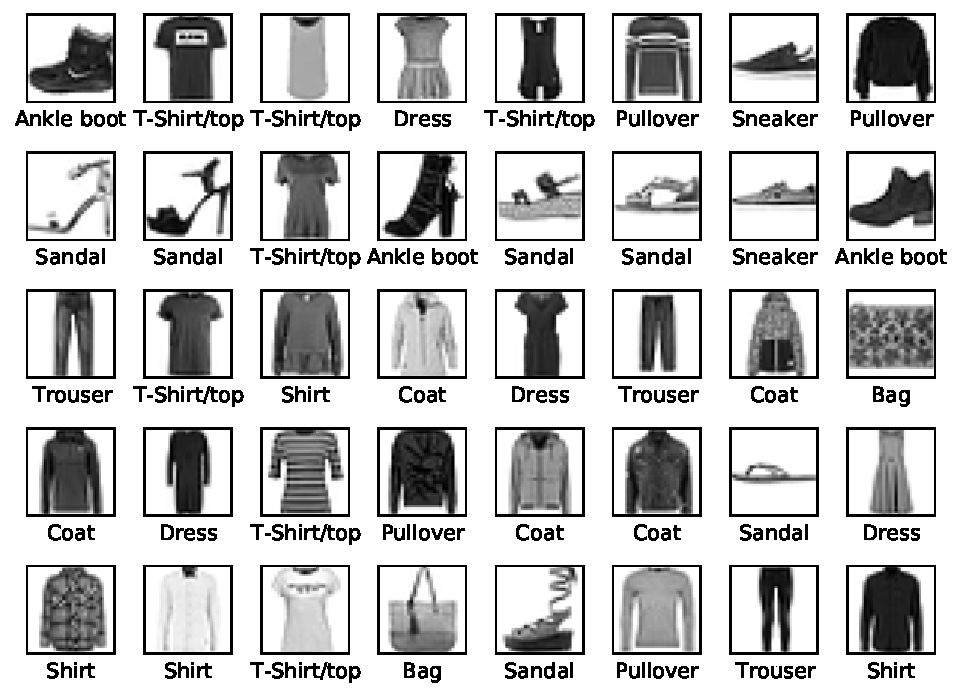
\includegraphics[width=0.7\textwidth]{chapters/Datasets/figures/Fashion_MNIST.pdf}
    \fonte{From the author (2021)}
    \label{fig:dataset_fashion_mnist}
\end{figure}


\section{CIFAR-10} \label{sec:cifar}
The \gls{CIFAR} datasets, \gls{CIFAR}-10 and \gls{CIFAR}-100, are two different subsets of the much larger 80 Million Tiny Images dataset, both are made of 60,000 (50,000 training and 10,000 testing) colored natural images of size $32{\times}32$ that were labeled by paid students to fit in a set of classes.

The images from \gls{CIFAR}-10 are divided into 10 classes with 6,000 images each, while \gls{CIFAR}-100 has 100 classes with 600 images each \cite{cifar2009}. For this document, only the \gls{CIFAR}-10 dataset was chosen for the experiments.

The \gls{CIFAR} datasets are another very popular choice for benchmarking neural networks, but given that they consist of colored images with increased resolution and more complex classes they offer considerably more challenge when compared to the \gls{MNIST} dataset. \autoref{fig:dataset_cifar10} shows examples of labeled samples taken from the \gls{CIFAR}-10 dataset.
\begin{figure}[hbt]
    \centering
    \caption{Labeled samples from CIFAR10 dataset}
    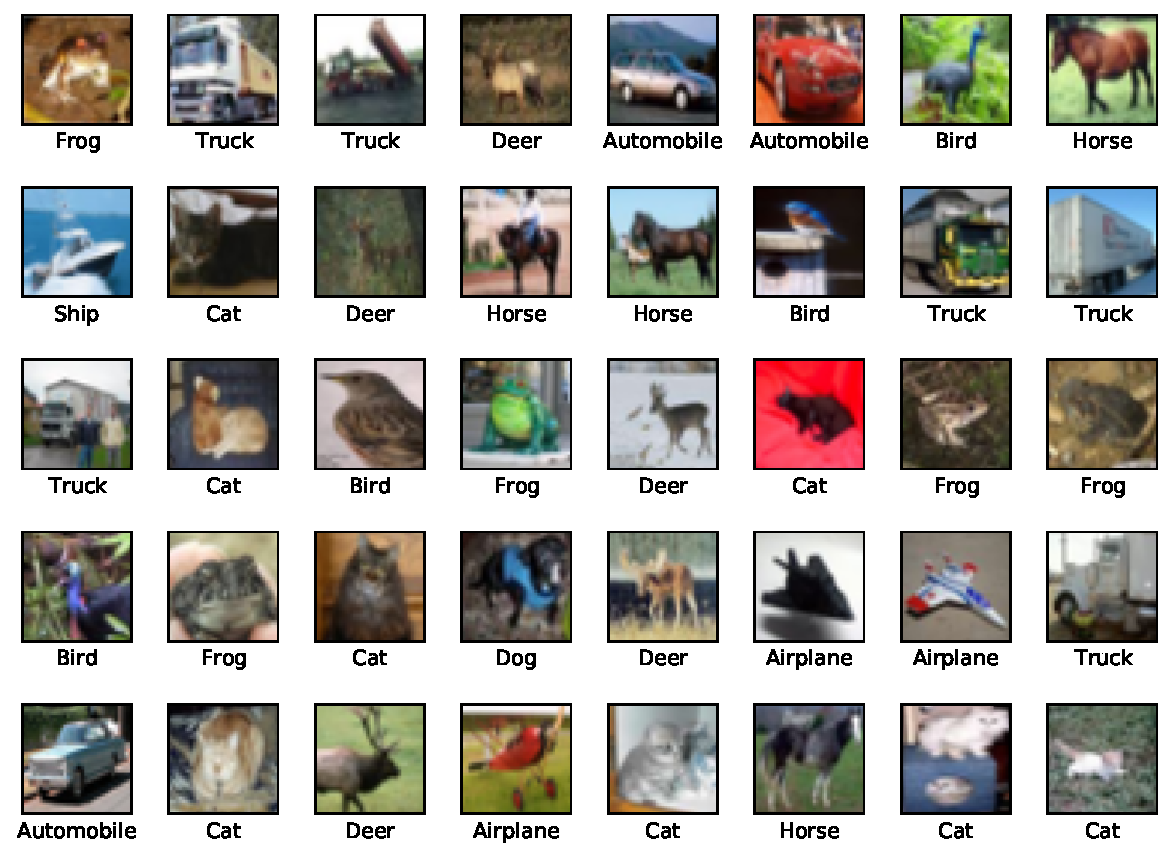
\includegraphics[width=0.7\textwidth]{chapters/Datasets/figures/CIFAR10.pdf}
    \fonte{From the author (2021)}
    \label{fig:dataset_cifar10}
\end{figure}



\section{Flowers} \label{sec:flowers}
The flowers dataset consists of $8,189$ high resolution images of 102 different categories of flowers, each category has from 40 to 250 different images \cite{flowers2008}. Samples from this dataset can be seen on \autoref{fig:dataset_flowers}

\begin{figure} [hbt]
    \centering
    \caption{Samples from the Flowers dataset}
    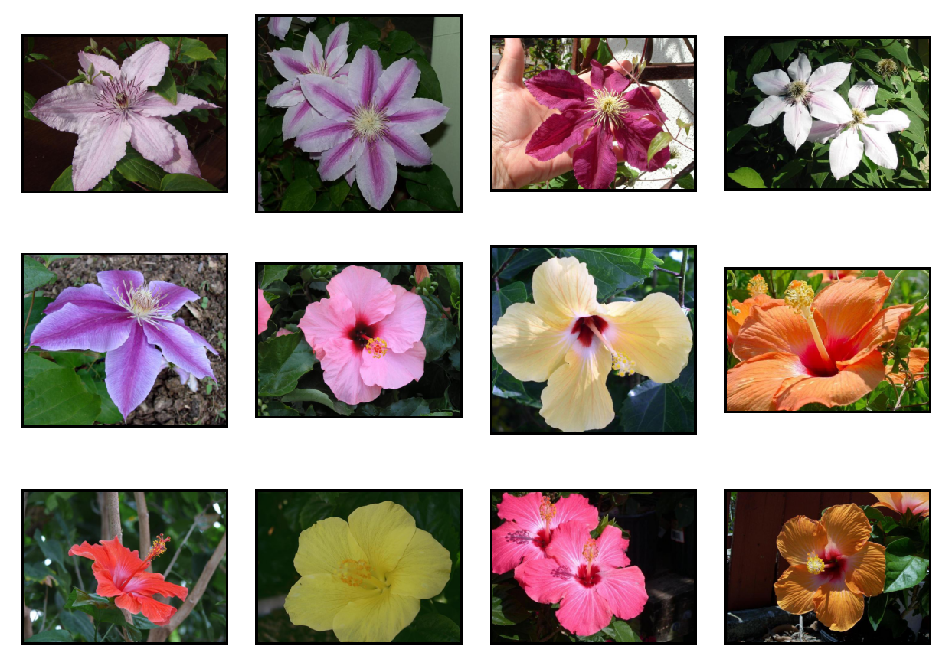
\includegraphics[width=0.8\textwidth]{chapters/Datasets/figures/Flowers.pdf}
    \fonte{From the author (2021)}
    \label{fig:dataset_flowers}
\end{figure}

\section{CelebA} \label{sec:celebA}
This is the largest dataset used in this document in terms of number of elements, it consists of $202,599$ pictures of faces of celebrities, all rescaled to size $178\times218$. All images are heavily annotated, having $40$ binary features (e.g. blonde hair, eyeglasses, wearing hat, young) and the positions of eyes, nose and mouth all labeled \cite{celebA2015}. However, for the purposes of this document the annotations will not be relevant. \autoref{fig:dataset_celeba} shows examples of pictures in this dataset.
\begin{figure}
    \centering
    \caption{Samples from the CelebA dataset}
    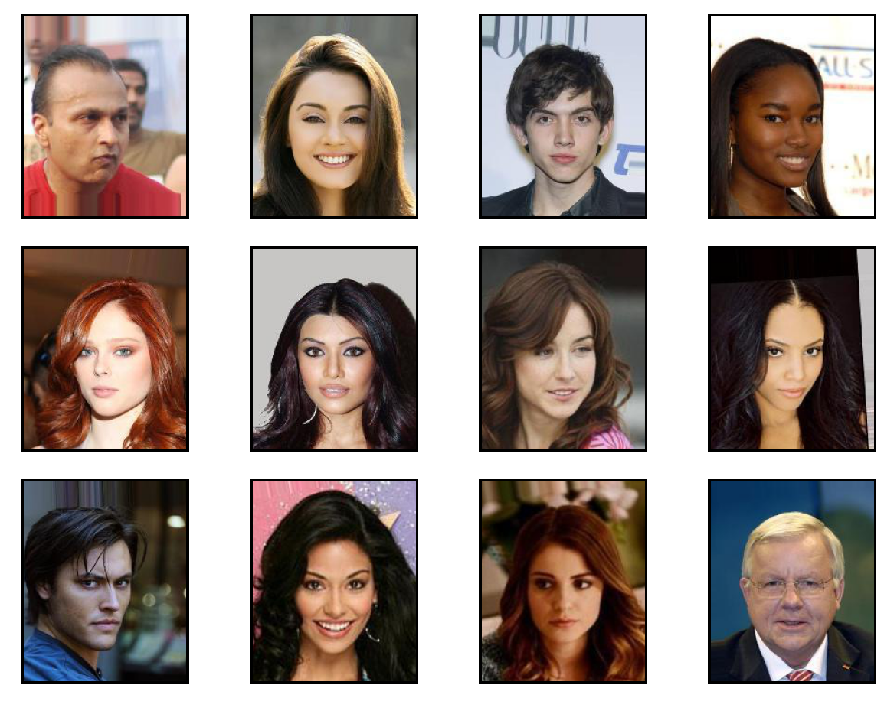
\includegraphics[width=0.8\textwidth]{chapters/Datasets/figures/CelebA.pdf}
    \fonte{From the author (2021)}
    \label{fig:dataset_celeba}
\end{figure}

\chapter{Datasets} \label{cha:datasets}
To understand the concepts explored in this document it is sometimes helpful to bring real world examples in order to represent the theoretical ideas in more familiar terms. This chapter will introduce the datasets relevant to this document, used for explaining the concepts, but mostly for performing the experiments that will be described in \autoref{cha:experiments}.

For any machine learning problem there is the desire to model something, some practical examples could be: how likely a person is to have a disease given a set of medical conditions; what type of animal an image represents; or what is the best move to make given a board position in chess. Whatever the underlying situation being modeled, it is necessary to have some data to build the model around.

This data can be obtained through self play (e.g. in Reinforcement Learning problems), but in the majority of cases it is given by a dataset. A dataset is simply a collection of samples from the situation being modeled, it does not contain all the possible values but, if sufficiently expansive, it should have enough samples to be a good representation of the distributions and particularities of the modeled situation. The goal of a dataset is to contain enough data, so that a machine learning algorithm trained on it can generalize well to data outside of it.

For neural networks a dataset is commonly divided into three groups: training, validation and test data. The training data is used in the learning process, it is what the network will see and will try to model, given this importance it is usually the largest chunk of a dataset. The validation data on the other hand is used to decide how to build the network and how to train the model, another way of saying this is that the training data is used to tune the network's parameters, while the validation data is used to tune the hyperparameters (see \autoref{sec:loss_&_gradient_descent}).

The validation process consists of training several models on the usually smaller validation data and seeing which set of hyperparameters produced the better results. One might wonder why would there be a need for this data and why not just use the training data instead? The main benefit of using a different set for validation is that validating on the training data has the risk of finding a set of hyperparameters that is particularly good on this data but that does not generalize well, using a separate validation data is a way to not overfit the hyperparameters to the training data and achieve better generalization.

The last chunk of a dataset, the test data, is used to validate the quality of the model and it's hability to generalize. This data should never be used to update either the parameters or hyperparameters, it should instead only be used as an evaluation tool, a way to estimate how well the model will perform on unseen data.

The next sections will explore the datasets relevant to the experiments made for this document. It is usual for datasets to already come separated into train and test data (the validation data is usually taken from a subset of the training data only if needed). This division will be mentioned for the described datasets, but it is relevant to note that any other divisions could also be obtained by combining and redistributing the data differently.


\section{MNIST} \label{sec:mnist}
\glsreset{MNIST}
Introduced in 1998 by \textcite{mnist1998}, the \gls{MNIST} is one of the most popular datasets in the field of machine learning, it's simplicity has made it a perfect choice as an introduction to deep learning and classification problems \cite{NN&DL2015}, but also as a benchmark for new techniques in serious research \textbf{--} some examples include \cite{dropout2012}, \cite{gans2014}, \cite{conditionalGAN2014} and \cite{adam2017}.

This dataset consists of 70,000 (60,000 training and 10,000 test) gray-scale images of handwritten digits, all images are of size $28{\times}28$ pixels and are labeled with the corresponding digit. The pixel values are inverted, this means that the strength of the strokes are represented with white pixels (values close to 255) against a black background (pixel value 0), this is however just how the data is represented numerically, for visualization purposes it is better to invert the colors as seen on \autoref{fig:dataset_mnist} \textbf{--} This figure shows some samples from this dataset along with the corresponding label.
\begin{figure}[hbt]
    \centering
    \caption{Labeled samples from the MNIST dataset}
    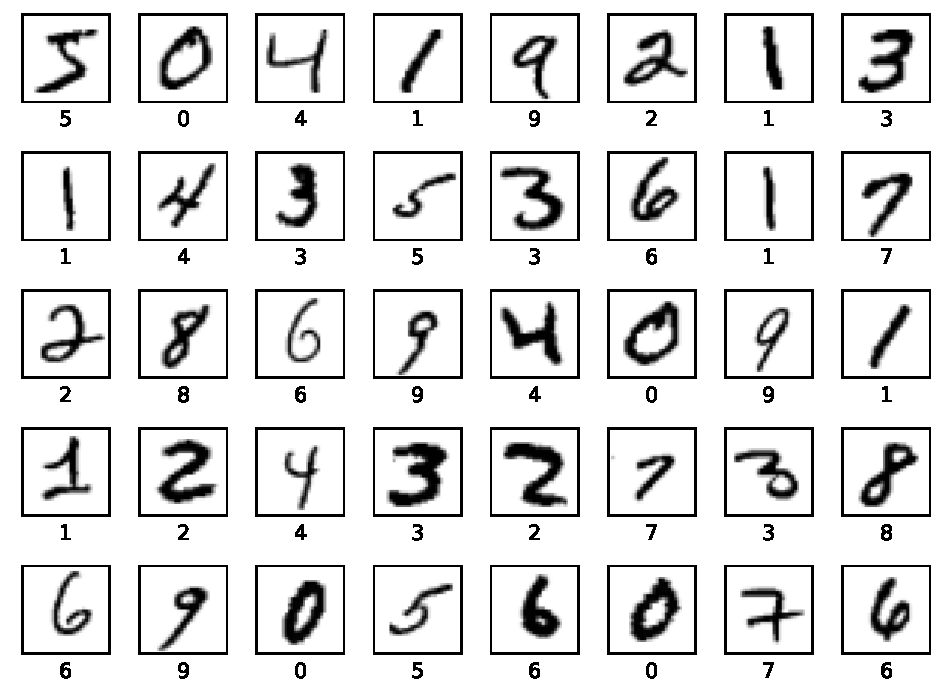
\includegraphics[width=0.6\textwidth]{chapters/Datasets/figures/MNIST.pdf}
    \fonte{From the author (2021)}
    \label{fig:dataset_mnist}
\end{figure}


\section{Fashion MNIST} \label{sec:fashion_mnist}
The simplicity of the \gls{MNIST} dataset makes it a very natural choice for benchmarking a Neural Network, however the data that it represents is also very simplistic \textbf{--} \textcite{mnistSOTA2013} were able to achieve a classification error lower than 0.3\% on the test set. The fact that \gls{MNIST} can be too easy has raised some questions about the usefulness of this dataset in benchmarking methods that scale to more complex tasks.

In response to these questions \textcite{fashionMNIST2017} proposed the Fashion MNIST dataset, arguing that \gls{MNIST} is too easy and cannot represent modern computer vision problems. Their goal was to replace \gls{MNIST} with a more robust dataset, without losing the simplicity of use that made the original so popular in the first place.

The Fashion MNIST dataset has all the same properties of \gls{MNIST}, it consists of 70,000 (60,000 training and 10,000 testing) $28{\times}28$ gray-scale images labelled from 0 to 9. The images however do not represent handwritten digits, they are instead preprocessed pictures of clothing items from the Zalando fashion company \cite{fashionMNIST2017}, the labels directly map to the type of clothing represented. Just like in \gls{MNIST}, the pixel values for the images are also inverted, the authors have made an effort to make the change of datasets as simple as just changing the link to get the files.

\autoref{fig:dataset_fashion_mnist} shows some labeled samples from this dataset, the pixel values are inverted for better visualization.
\begin{figure}[hbt]
    \centering
    \caption{Labeled samples from the Fashion MNIST dataset}
    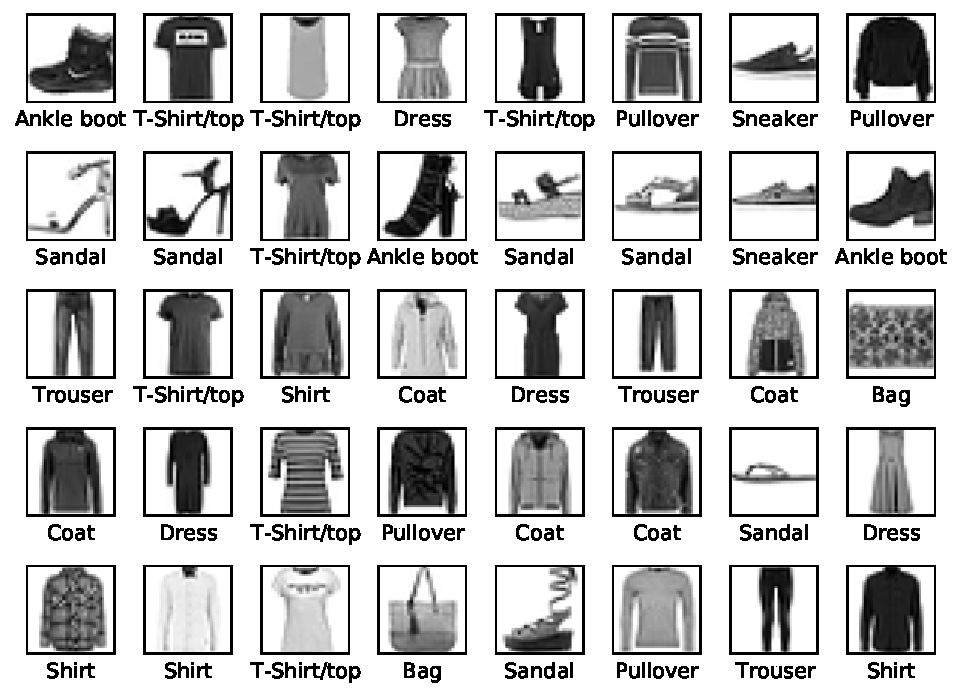
\includegraphics[width=0.7\textwidth]{chapters/Datasets/figures/Fashion_MNIST.pdf}
    \fonte{From the author (2021)}
    \label{fig:dataset_fashion_mnist}
\end{figure}


\section{CIFAR-10} \label{sec:cifar}
The \gls{CIFAR} datasets, \gls{CIFAR}-10 and \gls{CIFAR}-100, are two different subsets of the much larger 80 Million Tiny Images dataset, both are made of 60,000 (50,000 training and 10,000 testing) colored natural images of size $32{\times}32$ that were labeled by paid students to fit in a set of classes.

The images from \gls{CIFAR}-10 are divided into 10 classes with 6,000 images each, while \gls{CIFAR}-100 has 100 classes with 600 images each \cite{cifar2009}. For this document, only the \gls{CIFAR}-10 dataset was chosen for the experiments.

The \gls{CIFAR} datasets are another very popular choice for benchmarking neural networks, but given that they consist of colored images with increased resolution and more complex classes they offer considerably more challenge when compared to the \gls{MNIST} dataset. \autoref{fig:dataset_cifar10} shows examples of labeled samples taken from the \gls{CIFAR}-10 dataset.
\begin{figure}[hbt]
    \centering
    \caption{Labeled samples from CIFAR10 dataset}
    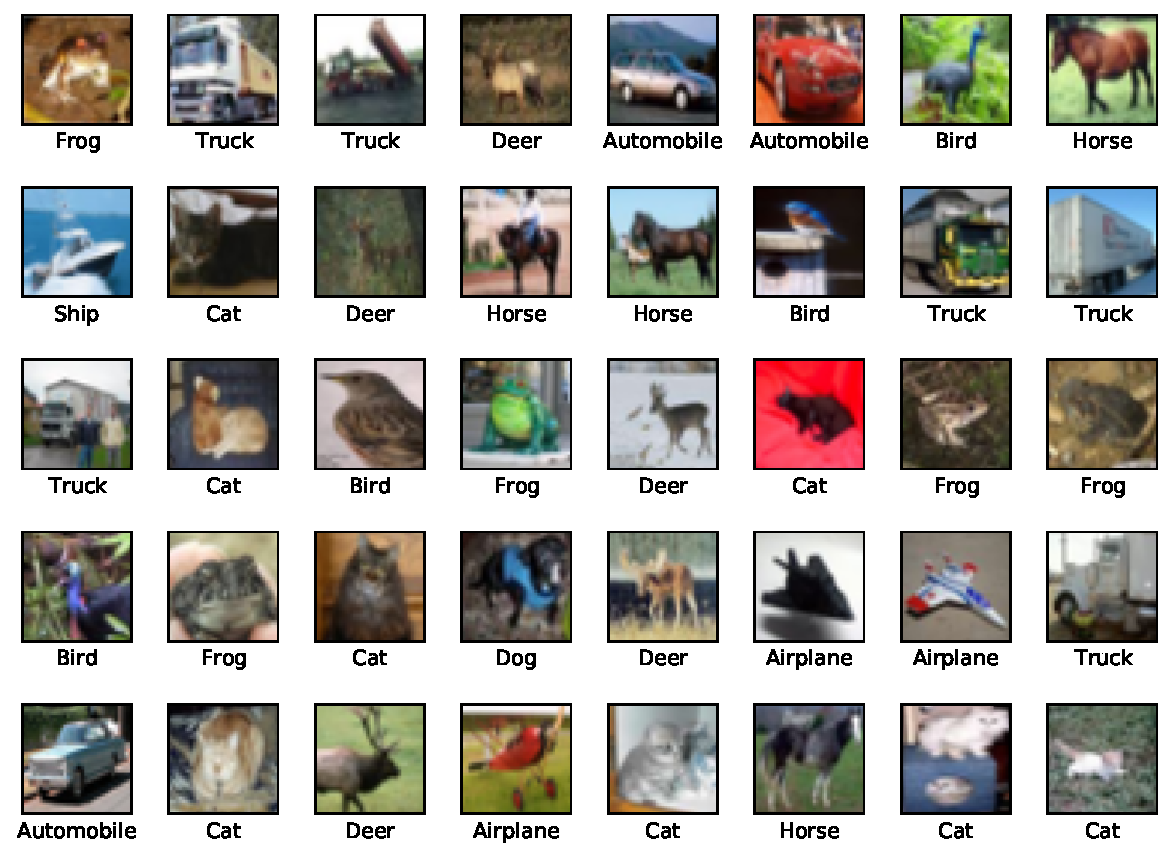
\includegraphics[width=0.7\textwidth]{chapters/Datasets/figures/CIFAR10.pdf}
    \fonte{From the author (2021)}
    \label{fig:dataset_cifar10}
\end{figure}



\section{Flowers} \label{sec:flowers}
The flowers dataset consists of $8,189$ high resolution images of 102 different categories of flowers, each category has from 40 to 250 different images \cite{flowers2008}. Samples from this dataset can be seen on \autoref{fig:dataset_flowers}

\begin{figure} [hbt]
    \centering
    \caption{Samples from the Flowers dataset}
    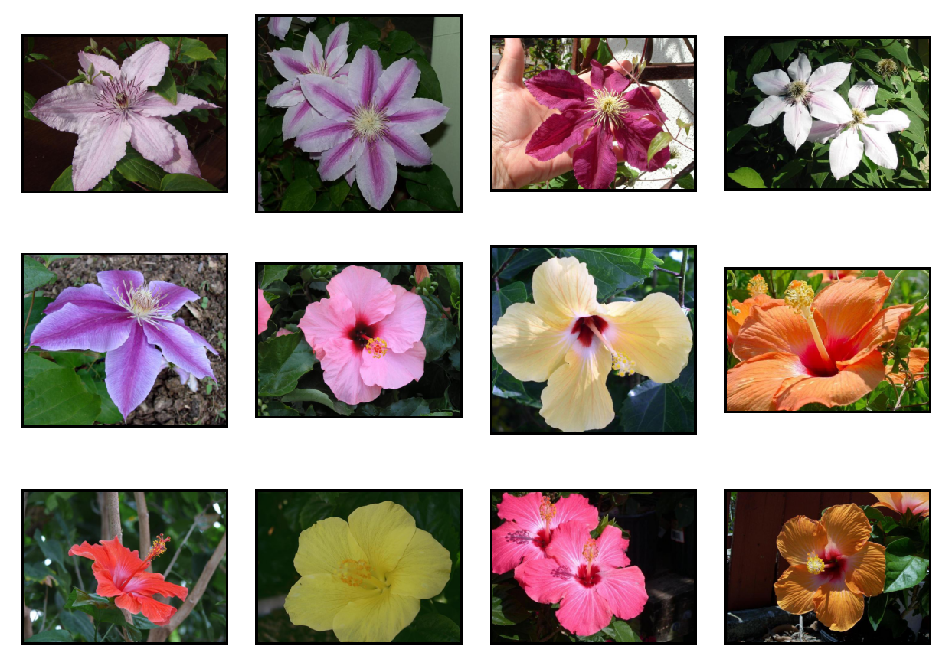
\includegraphics[width=0.8\textwidth]{chapters/Datasets/figures/Flowers.pdf}
    \fonte{From the author (2021)}
    \label{fig:dataset_flowers}
\end{figure}

\section{CelebA} \label{sec:celebA}
This is the largest dataset used in this document in terms of number of elements, it consists of $202,599$ pictures of faces of celebrities, all rescaled to size $178\times218$. All images are heavily annotated, having $40$ binary features (e.g. blonde hair, eyeglasses, wearing hat, young) and the positions of eyes, nose and mouth all labeled \cite{celebA2015}. However, for the purposes of this document the annotations will not be relevant. \autoref{fig:dataset_celeba} shows examples of pictures in this dataset.
\begin{figure}
    \centering
    \caption{Samples from the CelebA dataset}
    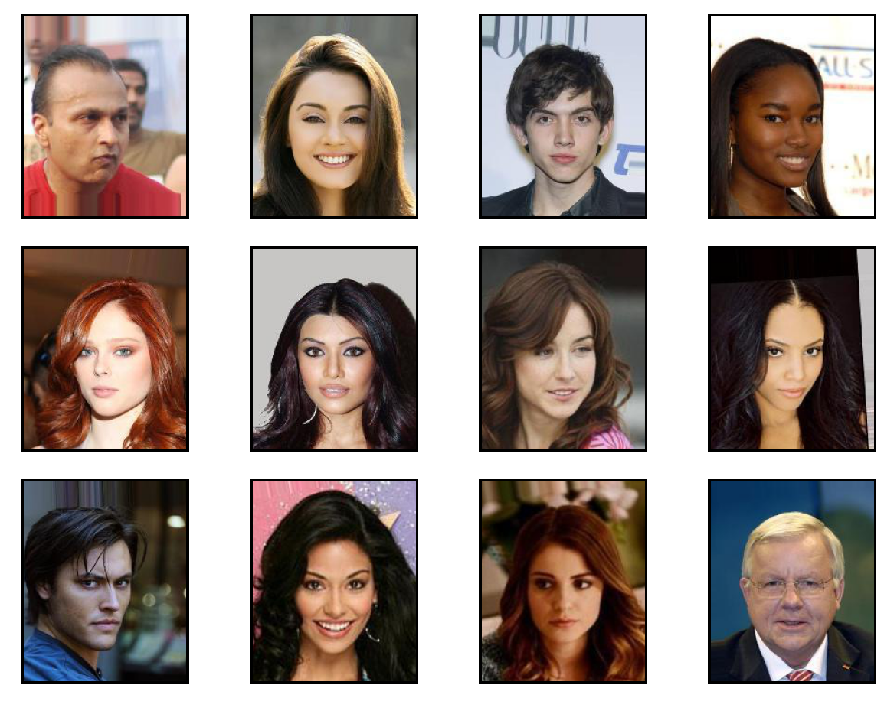
\includegraphics[width=0.8\textwidth]{chapters/Datasets/figures/CelebA.pdf}
    \fonte{From the author (2021)}
    \label{fig:dataset_celeba}
\end{figure}

\chapter{Datasets} \label{cha:datasets}
To understand the concepts explored in this document it is sometimes helpful to bring real world examples in order to represent the theoretical ideas in more familiar terms. This chapter will introduce the datasets relevant to this document, used for explaining the concepts, but mostly for performing the experiments that will be described in \autoref{cha:experiments}.

For any machine learning problem there is the desire to model something, some practical examples could be: how likely a person is to have a disease given a set of medical conditions; what type of animal an image represents; or what is the best move to make given a board position in chess. Whatever the underlying situation being modeled, it is necessary to have some data to build the model around.

This data can be obtained through self play (e.g. in Reinforcement Learning problems), but in the majority of cases it is given by a dataset. A dataset is simply a collection of samples from the situation being modeled, it does not contain all the possible values but, if sufficiently expansive, it should have enough samples to be a good representation of the distributions and particularities of the modeled situation. The goal of a dataset is to contain enough data, so that a machine learning algorithm trained on it can generalize well to data outside of it.

For neural networks a dataset is commonly divided into three groups: training, validation and test data. The training data is used in the learning process, it is what the network will see and will try to model, given this importance it is usually the largest chunk of a dataset. The validation data on the other hand is used to decide how to build the network and how to train the model, another way of saying this is that the training data is used to tune the network's parameters, while the validation data is used to tune the hyperparameters (see \autoref{sec:loss_&_gradient_descent}).

The validation process consists of training several models on the usually smaller validation data and seeing which set of hyperparameters produced the better results. One might wonder why would there be a need for this data and why not just use the training data instead? The main benefit of using a different set for validation is that validating on the training data has the risk of finding a set of hyperparameters that is particularly good on this data but that does not generalize well, using a separate validation data is a way to not overfit the hyperparameters to the training data and achieve better generalization.

The last chunk of a dataset, the test data, is used to validate the quality of the model and it's hability to generalize. This data should never be used to update either the parameters or hyperparameters, it should instead only be used as an evaluation tool, a way to estimate how well the model will perform on unseen data.

The next sections will explore the datasets relevant to the experiments made for this document. It is usual for datasets to already come separated into train and test data (the validation data is usually taken from a subset of the training data only if needed). This division will be mentioned for the described datasets, but it is relevant to note that any other divisions could also be obtained by combining and redistributing the data differently.


\section{MNIST} \label{sec:mnist}
\glsreset{MNIST}
Introduced in 1998 by \textcite{mnist1998}, the \gls{MNIST} is one of the most popular datasets in the field of machine learning, it's simplicity has made it a perfect choice as an introduction to deep learning and classification problems \cite{NN&DL2015}, but also as a benchmark for new techniques in serious research \textbf{--} some examples include \cite{dropout2012}, \cite{gans2014}, \cite{conditionalGAN2014} and \cite{adam2017}.

This dataset consists of 70,000 (60,000 training and 10,000 test) gray-scale images of handwritten digits, all images are of size $28{\times}28$ pixels and are labeled with the corresponding digit. The pixel values are inverted, this means that the strength of the strokes are represented with white pixels (values close to 255) against a black background (pixel value 0), this is however just how the data is represented numerically, for visualization purposes it is better to invert the colors as seen on \autoref{fig:dataset_mnist} \textbf{--} This figure shows some samples from this dataset along with the corresponding label.
\begin{figure}[hbt]
    \centering
    \caption{Labeled samples from the MNIST dataset}
    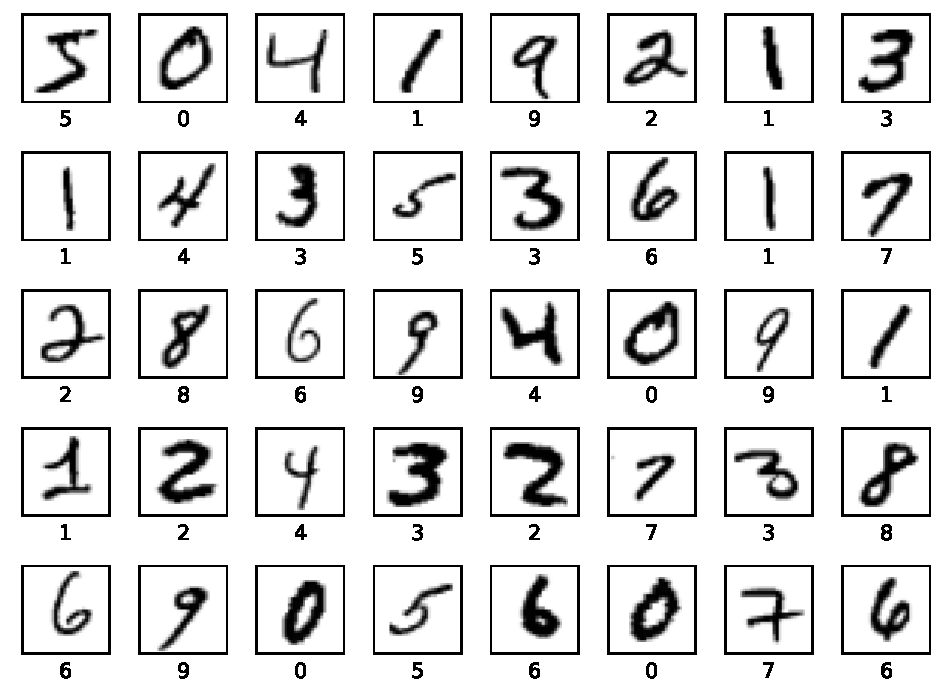
\includegraphics[width=0.6\textwidth]{chapters/Datasets/figures/MNIST.pdf}
    \fonte{From the author (2021)}
    \label{fig:dataset_mnist}
\end{figure}


\section{Fashion MNIST} \label{sec:fashion_mnist}
The simplicity of the \gls{MNIST} dataset makes it a very natural choice for benchmarking a Neural Network, however the data that it represents is also very simplistic \textbf{--} \textcite{mnistSOTA2013} were able to achieve a classification error lower than 0.3\% on the test set. The fact that \gls{MNIST} can be too easy has raised some questions about the usefulness of this dataset in benchmarking methods that scale to more complex tasks.

In response to these questions \textcite{fashionMNIST2017} proposed the Fashion MNIST dataset, arguing that \gls{MNIST} is too easy and cannot represent modern computer vision problems. Their goal was to replace \gls{MNIST} with a more robust dataset, without losing the simplicity of use that made the original so popular in the first place.

The Fashion MNIST dataset has all the same properties of \gls{MNIST}, it consists of 70,000 (60,000 training and 10,000 testing) $28{\times}28$ gray-scale images labelled from 0 to 9. The images however do not represent handwritten digits, they are instead preprocessed pictures of clothing items from the Zalando fashion company \cite{fashionMNIST2017}, the labels directly map to the type of clothing represented. Just like in \gls{MNIST}, the pixel values for the images are also inverted, the authors have made an effort to make the change of datasets as simple as just changing the link to get the files.

\autoref{fig:dataset_fashion_mnist} shows some labeled samples from this dataset, the pixel values are inverted for better visualization.
\begin{figure}[hbt]
    \centering
    \caption{Labeled samples from the Fashion MNIST dataset}
    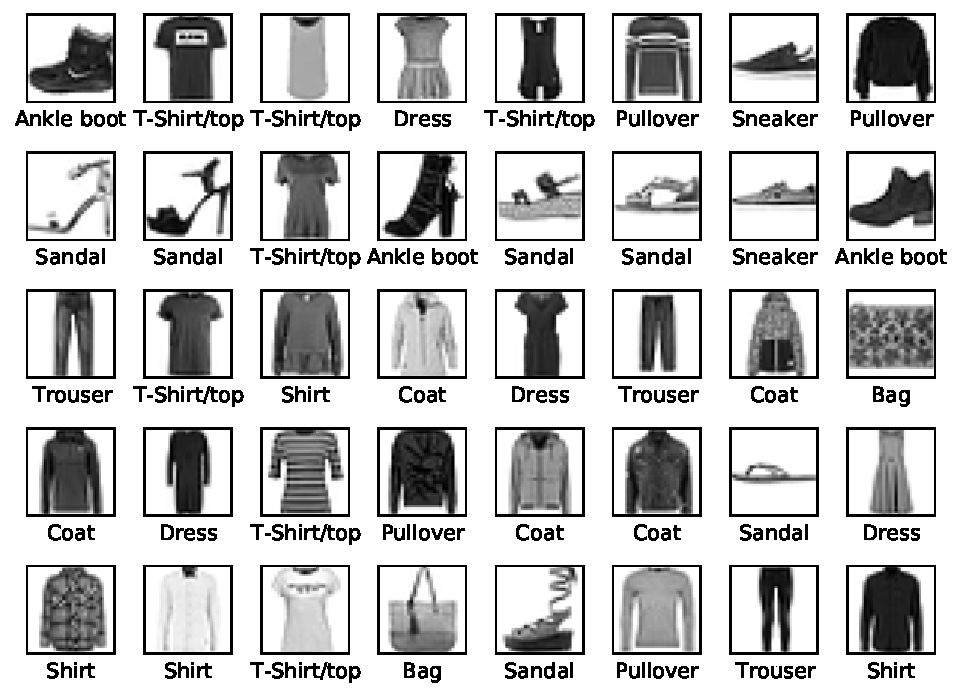
\includegraphics[width=0.7\textwidth]{chapters/Datasets/figures/Fashion_MNIST.pdf}
    \fonte{From the author (2021)}
    \label{fig:dataset_fashion_mnist}
\end{figure}


\section{CIFAR-10} \label{sec:cifar}
The \gls{CIFAR} datasets, \gls{CIFAR}-10 and \gls{CIFAR}-100, are two different subsets of the much larger 80 Million Tiny Images dataset, both are made of 60,000 (50,000 training and 10,000 testing) colored natural images of size $32{\times}32$ that were labeled by paid students to fit in a set of classes.

The images from \gls{CIFAR}-10 are divided into 10 classes with 6,000 images each, while \gls{CIFAR}-100 has 100 classes with 600 images each \cite{cifar2009}. For this document, only the \gls{CIFAR}-10 dataset was chosen for the experiments.

The \gls{CIFAR} datasets are another very popular choice for benchmarking neural networks, but given that they consist of colored images with increased resolution and more complex classes they offer considerably more challenge when compared to the \gls{MNIST} dataset. \autoref{fig:dataset_cifar10} shows examples of labeled samples taken from the \gls{CIFAR}-10 dataset.
\begin{figure}[hbt]
    \centering
    \caption{Labeled samples from CIFAR10 dataset}
    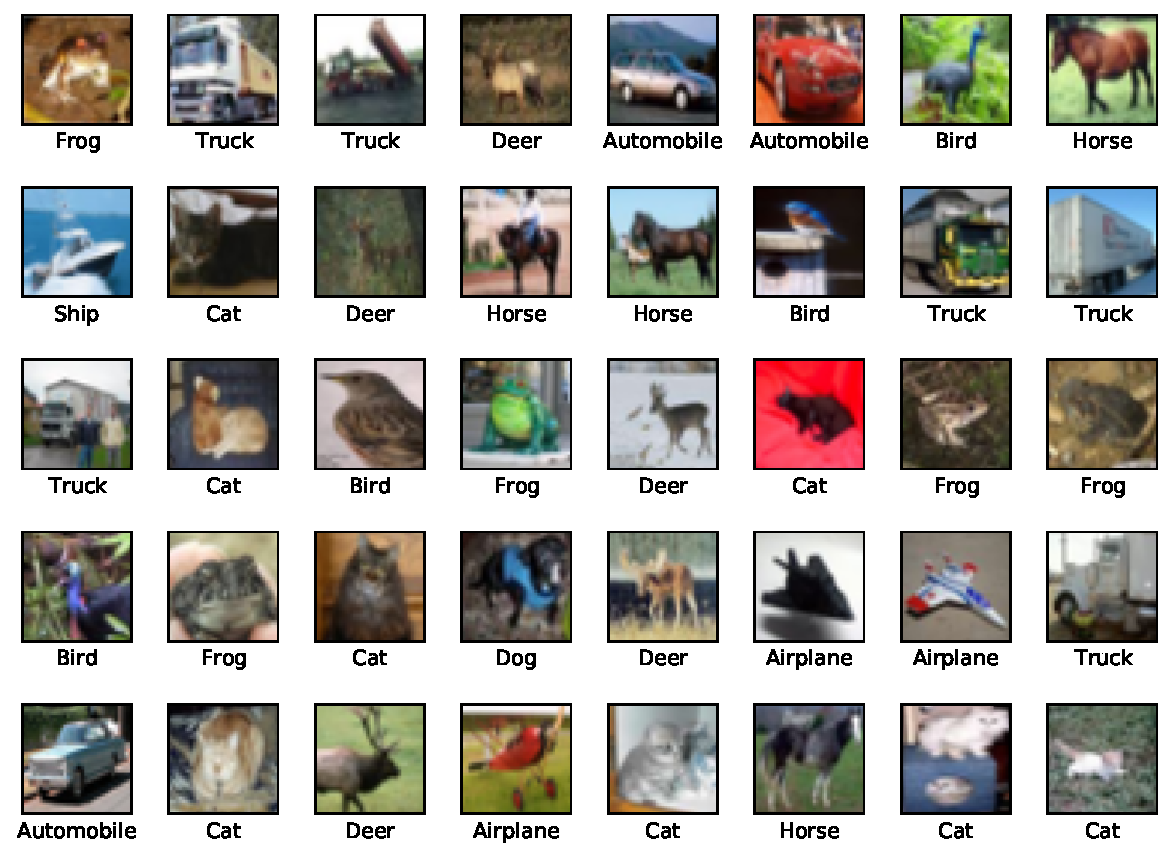
\includegraphics[width=0.7\textwidth]{chapters/Datasets/figures/CIFAR10.pdf}
    \fonte{From the author (2021)}
    \label{fig:dataset_cifar10}
\end{figure}



\section{Flowers} \label{sec:flowers}
The flowers dataset consists of $8,189$ high resolution images of 102 different categories of flowers, each category has from 40 to 250 different images \cite{flowers2008}. Samples from this dataset can be seen on \autoref{fig:dataset_flowers}

\begin{figure} [hbt]
    \centering
    \caption{Samples from the Flowers dataset}
    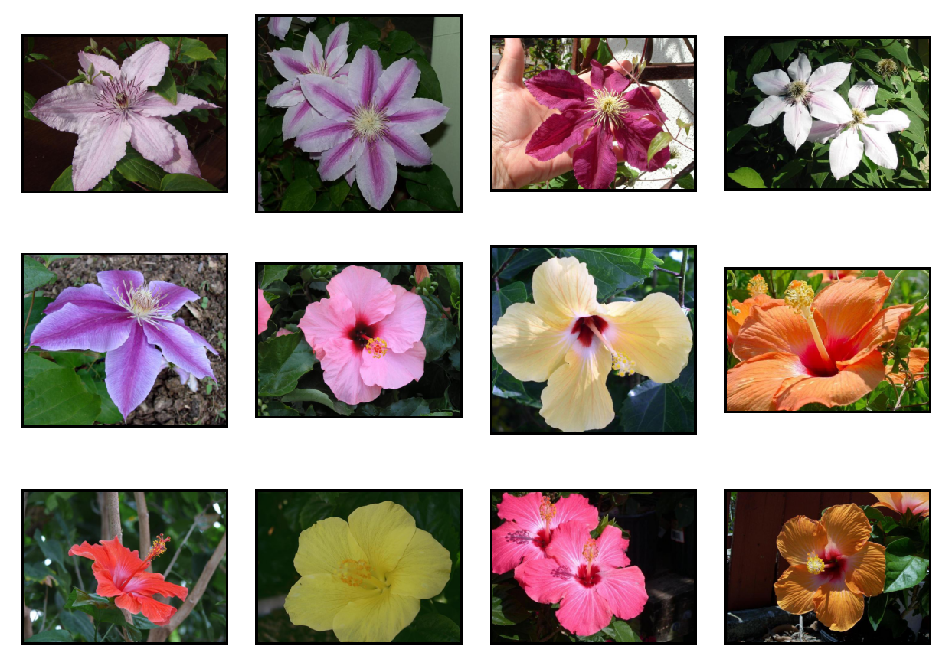
\includegraphics[width=0.8\textwidth]{chapters/Datasets/figures/Flowers.pdf}
    \fonte{From the author (2021)}
    \label{fig:dataset_flowers}
\end{figure}

\section{CelebA} \label{sec:celebA}
This is the largest dataset used in this document in terms of number of elements, it consists of $202,599$ pictures of faces of celebrities, all rescaled to size $178\times218$. All images are heavily annotated, having $40$ binary features (e.g. blonde hair, eyeglasses, wearing hat, young) and the positions of eyes, nose and mouth all labeled \cite{celebA2015}. However, for the purposes of this document the annotations will not be relevant. \autoref{fig:dataset_celeba} shows examples of pictures in this dataset.
\begin{figure}
    \centering
    \caption{Samples from the CelebA dataset}
    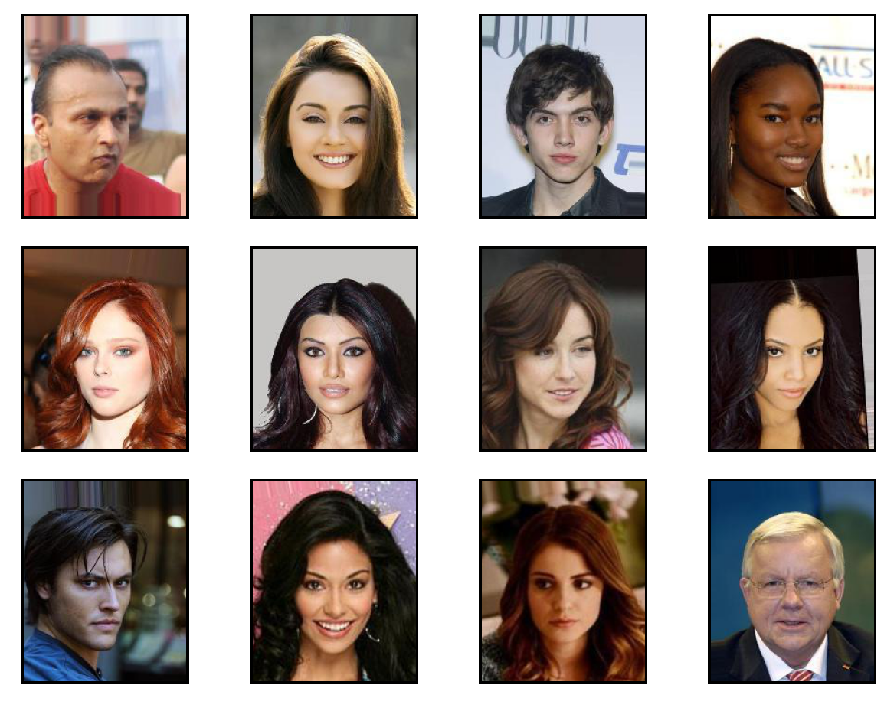
\includegraphics[width=0.8\textwidth]{chapters/Datasets/figures/CelebA.pdf}
    \fonte{From the author (2021)}
    \label{fig:dataset_celeba}
\end{figure}

